% The memoria in the EPS class tfgtfmthesisuam, version 3.2 as the TFG platform distributes it, which is read from tfgtfmthesisuam/ and used unchanged. The class marks the cover, the first and the last page of the body and the blank pages with invisible text, from which TFGTool counts the 40 pages. This file holds the options of the class, the data of the cover and the order of the chapters; sections/ holds the text, one file per chapter.
\documentclass[epsbased, tfg, english, covers, final, overleaf, nonelo]{tfgtfmthesisuam}

% What the text uses and the class does not load.
\usepackage{mathtools}
\usepackage{booktabs}
\usepackage{array}
% The range over the seeds that follows a mean difference in a table, set one size smaller so that the mean is read first.
\newcommand{\seedrange}[2]{{\footnotesize[$#1$, $#2$]}}
% A page of floats alone only when they fill most of it, so that a figure and a table that together fill half a page go on a page with text instead of leaving the rest of their page empty.
\renewcommand{\floatpagefraction}{0.7}
% A page that is not full ends where its text ends. Otherwise every page is filled to the bottom, which stretches the space around the figures, the equations and the paragraphs of a page whose next heading or figure moved to the following page.
\raggedbottom
\usetikzlibrary{arrows.meta, decorations.pathreplacing}

% The data figures of the Results are drawn by pgfplots from the CSV files in figures/data, so that their text is set in the face of the thesis. The CSV files are written by code/ai-experiments/thesis_figures_2026_09/extract.py from the run directories. The three colors are those of the diagrams, and each partition keeps its color and its mark in every figure, so that the figures still read in black and white.
\usepackage{pgfplots}
\usepgfplotslibrary{groupplots, fillbetween}
\pgfplotsset{compat=1.18}
\definecolor{moeblue}{RGB}{49,101,156}
\definecolor{moegreen}{RGB}{84,130,53}
\definecolor{moeamber}{RGB}{176,124,0}
\pgfplotsset{
  table/col sep=comma,
  thesis/.style={
      scale only axis, font=\footnotesize, line width=0.5pt,
      tick label style={font=\footnotesize, /pgf/number format/assume math mode=true},
      every axis plot/.append style={line width=0.8pt},
      legend style={font=\footnotesize, draw=none, fill=none, inner sep=1pt, row sep=-1pt},
      legend cell align=left,
      /pgf/number format/1000 sep={,},
    },
  arm a/.style={moeamber, mark=*, mark size=1.2pt},
  arm b/.style={moeblue, mark=square*, mark size=1.1pt},
  arm c/.style={moegreen, mark=triangle*, mark size=1.5pt},
  arm f/.style={black!55, mark=diamond*, mark size=1.5pt},
  band/.style={opacity=0.18, draw=none},
}

% The class sets the caption of a table below it. This copy of its table environment, with the same three arguments, sets it above, where tables usually carry it.
\makeatletter
\renewenvironment{table}[3][]
{%
  \abovecaptionskip=0.5\myem
  \belowcaptionskip=0pt
  \@float{table}[htbp]%
    \captionsetup{position=top}%
    \ifx&#1&\caption{#3}\else\caption[#1]{#3}\fi
    \ifx&#2&\else\label{#2}\fi
    \centering
}
{%
  \end@float
}
\makeatother

% The addresses in the bibliography are set in the face of the text, as the arXiv identifiers are.
\urlstyle{same}
% Paths and commands in typewriter that may break at a slash or a dot, for the reproduction appendix.
\DeclareUrlCommand\code{\urlstyle{tt}}

% The class's equation typesets the spaces of its own definition. The one at its start can take a line of its own when the text before the display fills its line, which leaves an empty line above the display; the ones at its end indent the line after the display. The first hook keeps the space on the line of the text, and the second removes the spaces at the end, so that a line such as ``where ...'' starts at the margin.
\makeatletter
\AddToHook{env/equation/begin}{\ifhmode\unskip\nobreak\fi}
\AddToHook{env/equation/after}{\loop\ifdim\lastskip>\z@\unskip\repeat}
\makeatother

% The names \cref writes. With the option english the class still gives cleveref its Spanish names, so the English ones are set here.
\crefname{chapter}{Chapter}{Chapters}
\Crefname{chapter}{Chapter}{Chapters}
\crefname{section}{Section}{Sections}
\Crefname{section}{Section}{Sections}
\crefname{subsection}{Section}{Sections}
\Crefname{subsection}{Section}{Sections}
\crefname{appendix}{Appendix}{Appendices}
\Crefname{appendix}{Appendix}{Appendices}
\crefname{figure}{Figure}{Figures}
\Crefname{figure}{Figure}{Figures}
\crefname{table}{Table}{Tables}
\Crefname{table}{Table}{Tables}
\crefname{equation}{Equation}{Equations}
\Crefname{equation}{Equation}{Equations}
% The class leaves the conjunctions between references in Spanish as well. cleveref sets them when the document begins, so they are replaced after that, in American English, with a comma before the last of three or more references and "to" in a range.
\AtBeginDocument{%
  \renewcommand{\crefpairconjunction}{ and\nobreakspace}%
  \renewcommand{\crefpairgroupconjunction}{ and\nobreakspace}%
  \renewcommand{\creflastconjunction}{, and\nobreakspace}%
  \renewcommand{\creflastgroupconjunction}{, and\nobreakspace}%
  \renewcommand{\crefrangeconjunction}{ to\nobreakspace}%
}

% The cover sets the title justified in a box that starts under "Bachelor thesis" and ends at the brown band, so a title longer than one line reaches the band, and the class leaves spaces before the first word. \ifcovertitle tells that box apart by its width, which the class keeps in \@poswttt and which no other place that prints the title has. There, \coverstart removes the spaces and sets the lines at the font's own spacing rather than the 1.3 of the text, so that three lines fit above the grey band, and \coverbreak ends a line. Everywhere else, on the title page, the copyright page and in the PDF's metadata, \coverstart does nothing and \coverbreak is a space.
\makeatletter
\newcommand{\ifcovertitle}{\ifdim\linewidth=\@poswttt\relax\expandafter\@firstoftwo\else\expandafter\@secondoftwo\fi}
\newcommand{\coverstart}{\ifcovertitle{\loop\ifdim\lastskip>\z@\unskip\repeat\linespread{1}\selectfont}{}}
\newcommand{\coverbreak}{\ifcovertitle{\newline}{\space}}
\makeatother
% The title registered on the platform, which the cover, the title page and the copyright page print whole; the footers carry the short form in brackets.
\title[How the Optimizer Shapes Routing]{\coverstart How the Optimizer Shapes Routing:\coverbreak Load Balancing, Specialization, and Stability\coverbreak in Mixture-of-Experts Language Models Trained with Muon}
\author{Marcos Hernanz Antón}
\advisor{Daniel Hernández Lobato}
\levelin{Ingeniería Informática}
\copyrightdate{\the\year}

\resumenfile{front/resumen}
\abstractfile{front/abstract}
% The class prints the keywords at the foot of the Abstract and the Resumen.
\keywords{Mixture of experts, load balancing, Muon, AdamW, optimization, routing, language models, deep learning}
\palabrasclave{Mezcla de expertos, equilibrado de carga, Muon, AdamW, optimización, enrutamiento, modelos de lenguaje, aprendizaje profundo}

% The metadata of the PDF, with the values the class gives them. The class sets them from the title page, which the option covers places after the cover, and by then hyperref has written them, so they are set here, before the first page.
\makeatletter
\pdfmetavalues{\@author}{\@titleaux}{Bachelor thesis}{\@auxkeywords, \@auxpalabrasclave}
\makeatother

% The cover prints these lines under the author. TFGTool looks there for the tutor's name as it is registered on the platform, so the advisor goes first, written the same way as in \advisor.
\coverdata
{
  Advisor: Daniel Hernández Lobato \\[1ex]
  Escuela Politécnica Superior \\
  Universidad Autónoma de Madrid \\
  C/ Francisco Tomás y Valiente, 11
}

\bibliographyconfig[ieeetr]{references}

% The class adds the contents entry of the bibliography after printing it, so the entry shows its last page. This copy of \thesisbibliography adds it on the first page instead.
\makeatletter
\renewcommand{\thesisbibliography}{%
  \if@bibliographymodebool
    \cleardoublepage\phantomsection\addcontentsline{toc}{chapter}{\bibname}%
    \bibliographystyle{\@bibstyleaux}%
    \bibliography{\@bibfileaux}%
  \fi
}
\makeatother

\begin{document}

% The body, in the usual order of an empirical paper: the setup that every experiment shares in the Method, one section per question in the Results, and the interpretation and the limits in the Discussion. The body that counts toward the 40 pages runs from the first page of the Introduction to the last of the Conclusions.
% !TEX root = ../main.tex
\chapter{Introduction}
\label{sec:introduction}

\section{Motivation}
\label{sec:introduction-motivation}
Large language models are neural networks trained to predict the next word of a text, and the largest have trillions of parameters. Most of the leading open models of 2026, such as DeepSeek-V4, Kimi K3, GLM-5.3, Qwen3.8-Flash-Next, and MiMo-V2.6, are based on the \emph{mixture-of-experts} (MoE) architecture \cite{deepseek2026v4, kimi2026k3, zai2026glm53, qiu2026qwennext, xiaomi2026mimov26}. In most of their layers, the feed-forward network is split into many smaller networks, called \emph{experts}. A small network called the \emph{router} sends each \emph{token}, a word or a piece of a word, to a few of the experts. Only these experts process it. An MoE model can therefore have many parameters while each token uses only a small fraction of them. This makes it much cheaper to train and to run than a dense model of the same size, which uses all its parameters for every token.

Two choices in how these models are trained are the subject of this thesis. The first is how the experts are kept equally busy, which does not happen on its own. A router trained without any correction tends to send most tokens to a few experts. These experts are then trained on more tokens and become even more attractive to the router, while the others stay idle \cite{shazeer2017outrageously}. Many current models prevent this with a small correction for each expert, called the \emph{bias}. After every training step, the bias is lowered if the expert received too many tokens and raised if it received too few \cite{wang2024lossfree}.

For each token, the router computes a score for every expert, adds the bias of each expert to its score, and sends the token to the few experts with the highest sum. An expert that receives high scores for most tokens therefore needs a lower bias than the others, so that it receives no more than its \emph{fair share} of the tokens. The fair share is what each expert would receive if all of them were equally busy. The more strongly the router favors some experts over others, the further apart their biases must be. We measure how hard the bias works by the \emph{span}, the largest minus the smallest bias in a layer.

The second choice is the \emph{optimizer}, the rule that turns the gradient of the loss into an update of the parameters. Until recently, most language models were trained with AdamW \cite{loshchilov2019decoupled}, a variant of the Adam optimizer \cite{kingma2015adam} that scales the update of each parameter separately from the others. Most of the leading open models of 2026 instead train nearly all their weight matrices with Muon \cite{jordan2024muon, liu2025moonlight} (\cref{tab:related-router}), which treats each matrix as a whole and gives it an update of a fixed size. Since the optimizer trains the router and the rest of the network, it shapes the scores that the bias has to correct. This thesis therefore studies how the choice of optimizer changes the work of the bias.

The labs that build these models disagree on which optimizer should train the router. DeepSeek-V4 and Kimi K3 train it with Muon, like their other weight matrices \cite{deepseek2026v4, kimi2026k3}, whereas Qwen3.8-Flash-Next and MiMo-V2.6 use AdamW for it \cite{qiu2026qwennext, xiaomi2026mimov26}. According to the Qwen3.8-Flash-Next report, Muon made the router unstable early in training and gave no clear gain later \cite{qiu2026qwennext}. The DeepSeek-V4 report also links the routing to the stability of training. The \emph{loss spikes} of DeepSeek-V4, sudden jumps of the loss, came with very large activations in the MoE layers, which the routing itself appears to make larger \cite{deepseek2026v4}. None of these reports compare the options under controlled conditions. Moreover, the few studies that compare optimizers in MoE models either train without the bias or do not measure what it does \cite{wang2026depth, lau2026symmetry, srivastava2026lossfree}. Therefore, no published measurement shows how Muon changes the work of the bias or which part of the network causes this change.

\section{Objectives and Approach}
\label{sec:introduction-objectives}
The objective of this thesis is to measure how the optimizer changes the work of the bias and the behavior of the router in MoE language models. We pursue it through three research questions.
\begin{itemize}
  \item \textbf{RQ1.} How does training with Muon instead of AdamW change the span of the bias, the routing, the loss, and how specialized the experts become?
  \item \textbf{RQ2.} Current models use one of three \emph{partitions}, or assignments of the optimizers: all parameters on AdamW, all on Muon, or all on Muon except the router. How do these three partitions behave when the learning rate is raised far above its tuned value, as in the stress test of the Qwen3.8-Flash-Next report \cite{qiu2026qwennext}?
  \item \textbf{RQ3.} Which group of parameters, when trained with Muon, causes the higher span that RQ1 finds, and through what mechanism?
\end{itemize}

To answer these questions, we trained small MoE language models of two sizes on educational web text. The smaller uses 55M parameters for each token out of 303M in total, and the larger 108M out of 496M\@. In each run, we chose which optimizer trained each group of parameters, so that the router, the experts, and the other parts of the network could be moved to Muon one at a time. In total, we trained 145 runs. Except for the tuning of the learning rates, every configuration had three random seeds. Runs with the same seed start from the same weights and see the same data, so we compare configurations seed by seed. We also fixed the comparisons of each experiment before training its runs.

\section{Findings and Contributions}
\label{sec:introduction-findings}
Muon reached a lower loss than AdamW and made the experts more specialized, but it also made the bias work harder. The span was higher at every seed: 0.137 against 0.105 averaged over the layers, and 0.194 against 0.084 in the first MoE layer, where the difference was largest. We had expected the opposite. With Muon, the size of the update of an expert does not depend on how many tokens it receives, which should weaken the tendency of busy experts to become busier. Our runs confirmed this independence, yet the span still rose. How much it rose depended on the learning rate of Muon, which our tuning had set to twice that of AdamW\@. At half this rate, which trained slightly better, about three quarters of the extra span of the first MoE layer disappeared. The span also stayed higher with a bias four times faster, with the balance loss of DeepSeek-V3, and on the larger model.

The optimizer of the router changed the span of the first MoE layer little. What mattered was the optimizer of the \emph{backbone}, which we define as every weight matrix except the routers, the embedding table, and the output head. When the whole backbone was trained with Muon, the inputs of the first router shared a direction. The mean cosine similarity between the inputs of two tokens was about 0.4, against 0.07 under AdamW\@. Through this direction, the router favored the same experts for every token, and the bias needed hundreds of steps to cancel this preference. Meanwhile, the busiest expert of the layer received four to seven times its fair share. This overload did not raise our loss, but it could slow down training when the experts sit on many devices. In an exploratory test of whether the shared direction causes the overload, we repeated the start of some runs with one change. We subtracted the mean input of the batch from the input of the first router, which removes the shared direction. The overload and most of the extra span disappeared, and the loss did not change. Muon on the routed experts alone, however, raised the span even more, without a strong shared direction, and we do not know how.

A router trained with AdamW was updated more along the shared direction than one trained with Muon. With this router, the loads shifted more during the warmup, and the loss was slightly higher. This does not support the reason that the Qwen3.8-Flash-Next report gives for putting the router on AdamW\@. Far above the tuned rates, no run diverged, but the loss of Muon rose more than that of AdamW.

Summing up, the contributions of this thesis are the following:
\begin{itemize}
  \item A paired measurement, at two model sizes, of how much harder the bias works under Muon than under AdamW.
  \item A breakdown of this effect by group of parameters and by learning rate.
  \item An explanation of the higher span of the first MoE layer, tested by removing the shared direction.
  \item Evidence on which optimizer should train the router when the rest of the network is trained with Muon.
  \item A stress test of the three partitions of RQ2 at up to 16 times their tuned learning rates.
\end{itemize}

\section{Structure of the Document}
\label{sec:introduction-structure}
\Cref{sec:background} presents the background, and \cref{sec:related-work} reviews the related work. \Cref{sec:method} describes the setup that the experiments share. \Cref{sec:results} reports the experiments, and \cref{sec:discussion} interprets them and states their limits. \Cref{sec:conclusions} summarizes the answers and proposes future work. \Crefrange{app:configuration}{app:reproduction} give every setting of the runs, additional results, and how to reproduce them.

% !TEX root = ../main.tex
\chapter{Background}
\label{sec:background}

This chapter introduces what is needed to follow the experiments. \Cref{sec:background-lm} describes how a language model is built and trained, and \cref{sec:background-moe} describes the mixture-of-experts layer that our models use. \Cref{sec:background-balancing} explains how its experts are kept equally busy, and \cref{sec:background-optimizers} presents the two optimizers that we compare. Finally, \cref{sec:background-instability} describes the instabilities of training.

\section{Language Models and the Transformer}
\label{sec:background-lm}
A language model predicts the next piece of a text from the text before it. The text is first split into \emph{tokens}, which are words or pieces of words. A tokenizer, such as byte-pair encoding \cite{sennrich2016bpe}, fixes a vocabulary of $V$ symbols, so that a text becomes a sequence of integers $x_1, x_2, \dots$ between 1 and $V$. Given the tokens $x_1, \dots, x_t$, the model outputs a probability for every symbol of the vocabulary to be the next token $x_{t+1}$. It is trained to give a high probability to the token that actually comes next \cite{bengio2003neural, radford2019language}. On a sequence of $T + 1$ tokens, this means minimizing the cross-entropy
\begin{equation}[eq:background-lm-loss]{}
  \mathcal{L}(\boldsymbol{\theta}) = -\frac{1}{T} \sum_{t=1}^{T} \log p_{\boldsymbol{\theta}}(x_{t+1} \mid x_1, \dots, x_t),
\end{equation}
where $\boldsymbol{\theta}$ denotes all the parameters of the model and $p_{\boldsymbol{\theta}}$ the probability that it assigns. A model that spreads its probability evenly over $n$ symbols, one of which is correct, has a loss of $\log n$. The exponential of the loss, called the \emph{perplexity}, can therefore be read as the number of candidates among which the model is still undecided. A model that knows nothing has a loss of $\log V \approx 9.7$ with our vocabulary of 16,384 symbols. Our small model ends near 3.2, as if each next token were one of about 25 equally likely candidates.

The parameters are trained by mini-batch gradient descent, like those of other neural networks \cite{goodfellow2016deep}. At every training \emph{step}, the loss of \cref{eq:background-lm-loss} is computed on a \emph{batch} of sequences. Backpropagation~\cite{rumelhart1986learning} then gives its gradient with respect to every parameter, and every parameter is moved against its gradient. In its simplest form, the step is $\boldsymbol{\theta} \leftarrow \boldsymbol{\theta} - \eta \nabla \mathcal{L}$, where the \emph{learning rate} $\eta$ sets the size of the step. The learning rate changes over training according to a \emph{schedule}, which usually raises it from zero over a first period called the \emph{warmup} and then lowers it toward the end. The rule that turns the gradients into an update of the parameters is called the \emph{optimizer} (\cref{sec:background-optimizers}). The \emph{validation loss}, the loss on text kept out of training, measures how well the model predicts new text.

\begin{figure}[The decoder-only Transformer]{fig:background-model}{The decoder-only Transformer of this thesis for one position of the sequence. Every sublayer reads the residual stream through a normalization layer and adds its output to it at the circle. Block 0 has a dense FFN, and every later block has the MoE layer of \cref{fig:moe-layer} in its place. The boxes in gray and the gains of every normalization layer are trained with AdamW in every run.}
  % The decoder-only Transformer of Section 2.1 for one position: the residual stream from the embedding table to the output head, with every sublayer reading it and adding its output back. Gray marks what AdamW trains in every run; blue marks the MoE layer of Figure 2.2.
\definecolor{moeblue}{RGB}{49,101,156}
\definecolor{moeamber}{RGB}{176,124,0}
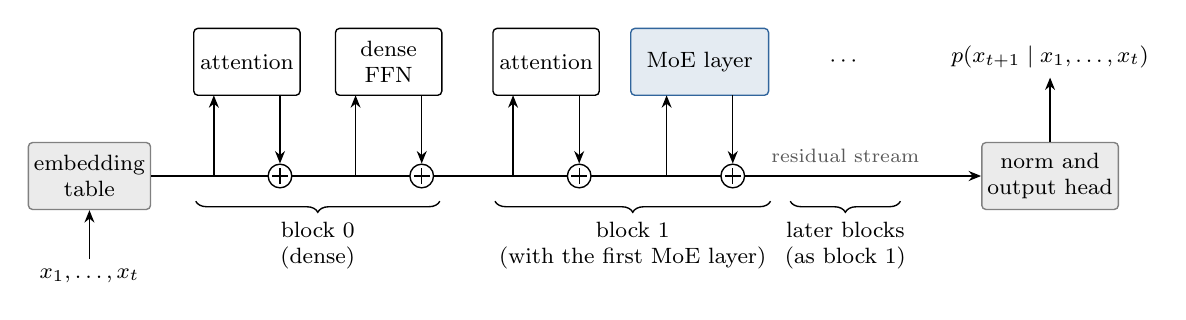
\begin{tikzpicture}[
    x=1cm, y=1cm, font=\footnotesize, line width=0.5pt,
    >={Stealth[length=4.5pt, width=3.6pt]},
    box/.style={draw, rounded corners=1.5pt, minimum height=0.85cm, inner sep=2pt, align=center},
    sub/.style={box, fill=white, minimum width=1.35cm},
    fixed/.style={box, draw=black!50, fill=black!8},
    moe/.style={box, draw=moeblue, fill=moeblue!13, minimum width=1.75cm},
    circ/.style={draw, circle, inner sep=0pt, minimum size=0.3cm, fill=white},
    tag/.style={font=\scriptsize, text=black!65},
  ]
  % The residual stream.
  \node[fixed] (emb) at (0.55, 0) {embedding\\table};
  \node[fixed] (head) at (12.75, 0) {norm and\\output head};
  \draw[->, line width=0.9pt] (emb) -- (head);
  \node[anchor=north] (tok) at (0.55, -1.05) {$x_1, \dots, x_t$};
  \draw[->] (tok) -- (emb);
  \node[anchor=south] (out) at (12.75, 1.25) {$p(x_{t+1} \mid x_1, \dots, x_t)$};
  \draw[->] (head) -- (out);

  % A sublayer reads the stream through a normalization layer and adds its output back.
  \newcommand{\sublayer}[4]{%
    \node[#3] at (#2, 1.45) {#4};
    \draw[->] (#2 - 0.42, 0) -- (#2 - 0.42, 1.025);
    \node[circ] (#1) at (#2 + 0.42, 0) {};
    \draw (#2 + 0.42 - 0.1, 0) -- (#2 + 0.42 + 0.1, 0);
    \draw (#2 + 0.42, -0.1) -- (#2 + 0.42, 0.1);
    \draw[->] (#2 + 0.42, 1.025) -- (#1);
  }
  \sublayer{plusa}{2.55}{sub}{attention}
  \sublayer{plusb}{4.35}{sub}{dense\\FFN}
  \sublayer{plusc}{6.35}{sub}{attention}
  \sublayer{plusd}{8.3}{moe}{MoE layer}
  \node at (10.15, 1.45) {$\cdots$};
  \node[tag, anchor=south] at (10.15, 0.05) {residual stream};

  % The blocks.
  \draw[decorate, decoration={brace, amplitude=4pt, mirror}] (1.9, -0.32) -- (5.0, -0.32)
    node[midway, below=4pt, align=center] {block 0\\(dense)};
  \draw[decorate, decoration={brace, amplitude=4pt, mirror}] (5.7, -0.32) -- (9.2, -0.32)
    node[midway, below=4pt, align=center] {block 1\\(with the first MoE layer)};
  \draw[decorate, decoration={brace, amplitude=4pt, mirror}] (9.45, -0.32) -- (10.85, -0.32)
    node[midway, below=4pt, align=center] {later blocks\\(as block 1)};
\end{tikzpicture}

\end{figure}

Our models are decoder-only Transformers \cite{vaswani2017attention, radford2019language}, drawn in \cref{fig:background-model}. An \emph{embedding table} gives every symbol of the vocabulary a vector of $d$ numbers, where $d$ is the \emph{width} of the model. Each position of the sequence thus starts as the vector of its token. A stack of \emph{blocks} then transforms these vectors. Each block adds its output to the vector of a position instead of replacing it, which is called a residual connection \cite{he2016resnet}. The vector of a position is therefore a running sum, called the \emph{residual stream}, to which every block writes. We call its value at a given point of the model the \emph{hidden state} of the token. After the last block, the \emph{output head}, a matrix with one row per symbol, gives every symbol a number. A softmax then turns these numbers into the probabilities of \cref{eq:background-lm-loss}.

Every block has two \emph{sublayers}, and a normalization layer rescales the hidden state before each of them reads it. Our models use RMSNorm \cite{zhang2019rmsnorm}, which divides the vector by the root mean square of its entries and multiplies it by learned \emph{gains}. The first sublayer, \emph{self-attention}, lets a position use the information of the positions before it. It multiplies the hidden state of every position by three weight matrices, which give a query, a key, and a value. A position weights itself and each earlier position by a softmax of the dot products of its query with their keys. It then takes the weighted mean of their values and maps it back to $d$ numbers with a fourth matrix, the output projection. The model does this in several \emph{heads} in parallel, on shorter vectors. The second sublayer, the \emph{feed-forward network} (FFN), is a small neural network with one hidden layer, applied to every position on its own and written out in \cref{eq:moe-expert}. Only the first block of our models, block 0, keeps this FFN, which we call \emph{dense}. Every later block replaces it with the mixture-of-experts layer of \cref{sec:background-moe}. Most of the parameters of a Transformer are in the weight matrices of these two sublayers, which Muon trains (\cref{sec:background-muon}).

\section{Mixture-of-Experts Layers}
\label{sec:background-moe}
A wider FFN usually gives a better model, but it also costs more computation for every token. A \emph{mixture-of-experts} (MoE) layer separates the number of parameters from the computation per token. It replaces the FFN with $E$ FFNs, called \emph{experts}, and a \emph{router} that sends each token to only $k$ of them. The number of parameters therefore grows with $E$, while the computation per token grows only with $k$. The router goes back to the gating network of Jacobs et~al.~\cite{jacobs1991adaptive}. Shazeer et~al.~\cite{shazeer2017outrageously} made the choice of the router \emph{sparse}, so that each token is processed by only a few experts. GShard and the Switch Transformer then put such a layer in place of the FFN of a Transformer \cite{lepikhin2021gshard, fedus2022switch}.

Our MoE layer, drawn in \cref{fig:moe-layer}, uses the DeepSeekMoE architecture \cite{dai2024deepseekmoe} with the routing function of DeepSeek-V3 \cite{deepseek2024v3}. DeepSeekMoE splits each expert into several narrower ones, so that a token can be routed to many more combinations of experts at the same cost. It also adds \emph{shared} experts, which every token uses, to capture knowledge that all tokens need. Let $\mathbf{x} \in \mathbb{R}^{d}$ denote the input of the layer for one token, which is its normalized hidden state. Our layer consists of $E$ routed experts $\operatorname{FFN}_1, \dots, \operatorname{FFN}_E$ and one shared expert $\operatorname{FFN}_{\mathrm{s}}$, and it computes
\begin{equation}[eq:moe-output]{}
  \mathbf{y} = \operatorname{FFN}_{\mathrm{s}}(\mathbf{x}) + \sum_{i \in \mathcal{T}(\mathbf{x})} g_i(\mathbf{x}) \operatorname{FFN}_i(\mathbf{x}),
\end{equation}
where $\mathcal{T}(\mathbf{x}) \subset \{1, \dots, E\}$ is the set of the $k$ routed experts selected for the token and the $g_i(\mathbf{x})$ are their mixing weights. Both come from the router.

\begin{figure}[The MoE layer for one token]{fig:moe-layer}{The MoE layer for one token. The router scores every expert with \cref{eq:moe-score}, selects $k$ of them by score plus bias with \cref{eq:moe-selection}, and weights their outputs with \cref{eq:moe-weights}. Only the shared expert and the highlighted routed experts, two in this drawing, are evaluated. No gradient flows through the dashed arrows, which carry the bias and the indices of the selected experts.}
  % The MoE layer of Section 2.1 for one token: the data path on the left, the router on the right. Dashed arrows carry what no gradient flows through.
\definecolor{moeblue}{RGB}{49,101,156}
\definecolor{moegreen}{RGB}{84,130,53}
\definecolor{moeamber}{RGB}{176,124,0}
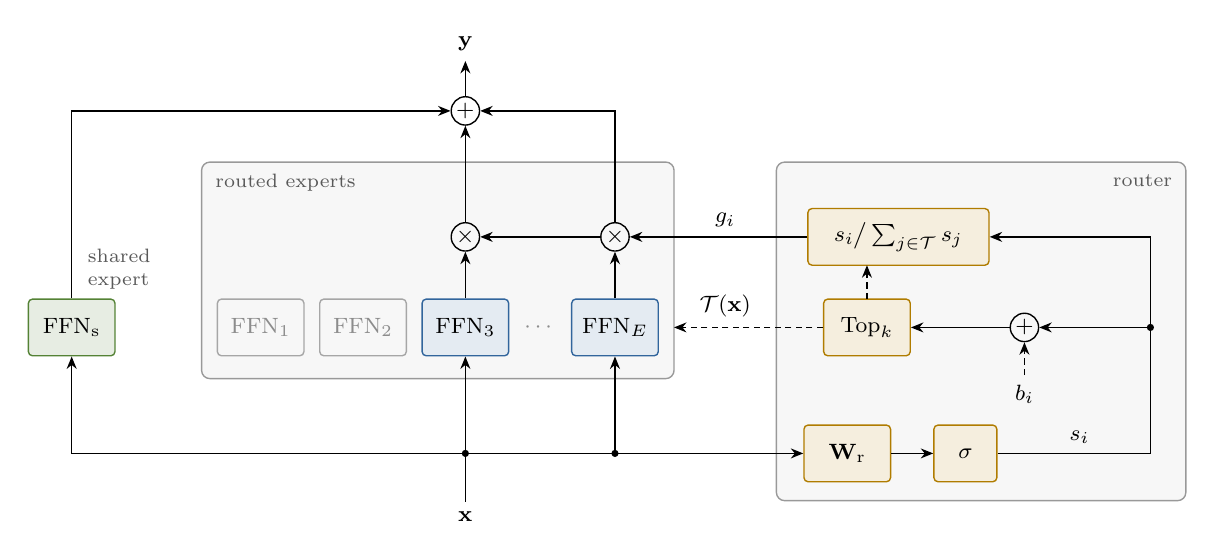
\begin{tikzpicture}[
    x=1cm, y=1cm, font=\footnotesize, line width=0.5pt,
    >={Stealth[length=4.5pt, width=3.6pt]},
    box/.style={draw, rounded corners=1.5pt, minimum width=1.1cm, minimum height=0.72cm, inner sep=1pt},
    shared/.style={box, draw=moegreen, fill=moegreen!14},
    active/.style={box, draw=moeblue, fill=moeblue!13},
    idle/.style={box, draw=black!35, text=black!45},
    op/.style={box, draw=moeamber, fill=moeamber!13},
    circ/.style={draw, circle, inner sep=0pt, minimum size=0.36cm},
    frame/.style={draw=black!40, rounded corners=3pt, fill=black!3},
    tag/.style={font=\scriptsize, text=black!65},
    nograd/.style={dashed, dash pattern=on 2.2pt off 1.6pt},
  ]
  % Frames first, so that everything else is drawn over them.
  \draw[frame] (1.15, 1.75) rectangle (7.15, 4.5);
  \draw[frame] (8.45, 0.2) rectangle (13.65, 4.5);
  \node[tag, anchor=north west] at (1.2, 4.47) {routed experts};
  \node[tag, anchor=north east] at (13.6, 4.47) {router};

  % Experts.
  \node[shared] (s) at (-0.5, 2.4) {$\operatorname{FFN}_{\mathrm{s}}$};
  \node[idle] (e1) at (1.9, 2.4) {$\operatorname{FFN}_1$};
  \node[idle] (e2) at (3.2, 2.4) {$\operatorname{FFN}_2$};
  \node[active] (e3) at (4.5, 2.4) {$\operatorname{FFN}_3$};
  \node[text=black!45] at (5.45, 2.4) {$\cdots$};
  \node[active] (eE) at (6.4, 2.4) {$\operatorname{FFN}_E$};
  \node[tag, anchor=west, align=left] at (-0.42, 3.14) {shared\\expert};

  % Input and the bus that carries it.
  \node (x) at (4.5, 0) {$\mathbf{x}$};
  \draw[->] (x) -- (e3);
  \draw[->] (4.5, 0.8) -| (s);
  \draw[->] (4.5, 0.8) -| (eE);
  \fill (4.5, 0.8) circle (1.3pt);
  \fill (6.4, 0.8) circle (1.3pt);

  % Router: scores.
  \node[op] (w) at (9.35, 0.8) {$\mathbf{W}_{\mathrm{r}}$};
  \node[op, minimum width=0.8cm] (sig) at (10.85, 0.8) {$\sigma$};
  \draw[->] (6.4, 0.8) -- (w);
  \draw[->] (w) -- (sig);
  % Router: selection on score plus bias.
  \node[circ] (plus) at (11.6, 2.4) {$+$};
  \node[op] (top) at (9.6, 2.4) {$\operatorname{Top}_k$};
  \node (b) at (11.6, 1.55) {$b_i$};
  \draw[->, nograd] (b) -- (plus);
  \draw[->] (sig) -- (13.2, 0.8) |- (plus);
  \node[anchor=south] at (12.3, 0.8) {$s_i$};
  \draw[->] (plus) -- (top);
  \draw[->, nograd] (top) -- (7.15, 2.4);
  \node[anchor=south] at (7.8, 2.4) {$\mathcal{T}(\mathbf{x})$};
  % Router: mixing weights from the scores alone.
  \node[op, minimum width=2.3cm] (norm) at (10.0, 3.55) {$s_i \big/ \sum_{j \in \mathcal{T}} s_j$};
  \draw[->] (13.2, 2.4) |- (norm);
  \fill (13.2, 2.4) circle (1.3pt);
  \draw[->, nograd] (9.6, 2.76) -- (9.6, 3.19);

  % Weighting and sum.
  \node[circ] (m3) at (4.5, 3.55) {$\times$};
  \node[circ] (mE) at (6.4, 3.55) {$\times$};
  \draw[->] (e3) -- (m3);
  \draw[->] (eE) -- (mE);
  \draw[->] (norm) -- (mE);
  \node[anchor=south] at (7.8, 3.55) {$g_i$};
  \draw[->] (mE) -- (m3);
  \node[circ] (sum) at (4.5, 5.15) {$+$};
  \draw[->] (m3) -- (sum);
  \draw[->] (s) |- (sum);
  \draw[->] (mE.north) |- (sum);
  \node (y) at (4.5, 6.0) {$\mathbf{y}$};
  \draw[->] (sum) -- (y);
\end{tikzpicture}

\end{figure}

The router is a matrix $\mathbf{W}_{\mathrm{r}} \in \mathbb{R}^{E \times d}$ whose row $\mathbf{w}_i$ gives the token a \emph{score} for expert $i$,
\begin{equation}[eq:moe-score]{}
  s_i = \sigma\bigl(\mathbf{w}_i^{\top} \mathbf{x}\bigr), \qquad i = 1, \dots, E,
\end{equation}
where $\sigma(z) = 1 / (1 + e^{-z})$ is the logistic sigmoid. Each score therefore lies in $(0, 1)$, as in logistic regression, and depends only on its own row of $\mathbf{W}_{\mathrm{r}}$. We call $\mathbf{w}_i^{\top} \mathbf{x}$ the \emph{logit} of expert $i$. The router then selects the $k$ experts with the largest values of $s_i + b_i$,
\begin{equation}[eq:moe-selection]{}
  \mathcal{T}(\mathbf{x}) = \operatorname{Top}_k \bigl( \{ s_i + b_i \}_{i=1}^{E} \bigr),
\end{equation}
where $\operatorname{Top}_k$ returns the indices of the $k$ largest elements and $\mathbf{b} \in \mathbb{R}^{E}$ holds the \emph{biases} of the experts, which keep the experts equally busy (\cref{sec:background-loss-free}). The mixing weights are the scores of the selected experts, normalized so that they sum to one,
\begin{equation}[eq:moe-weights]{}
  g_i = \frac{s_i}{\sum_{j \in \mathcal{T}(\mathbf{x})} s_j}, \qquad i \in \mathcal{T}(\mathbf{x}).
\end{equation}
The bias appears in \cref{eq:moe-selection} but not in \cref{eq:moe-weights}, so it changes which experts a token is sent to without changing how their outputs are weighted. Since the top-$k$ selection is not differentiable, the router receives gradient only through the mixing weights. Each token therefore contributes gradient only to the $k$ rows of $\mathbf{W}_{\mathrm{r}}$ that belong to its selected experts.

Each expert, routed or shared, is an FFN with the SwiGLU activation \cite{shazeer2020glu},
\begin{equation}[eq:moe-expert]{}
  \operatorname{FFN}_i(\mathbf{x}) = \mathbf{W}_i^{\mathrm{down}} \bigl( \operatorname{SiLU}(\mathbf{W}_i^{\mathrm{gate}} \mathbf{x}) \odot \mathbf{W}_i^{\mathrm{up}} \mathbf{x} \bigr),
\end{equation}
where $\mathbf{W}_i^{\mathrm{gate}}, \mathbf{W}_i^{\mathrm{up}} \in \mathbb{R}^{d_{\mathrm{e}} \times d}$ and $\mathbf{W}_i^{\mathrm{down}} \in \mathbb{R}^{d \times d_{\mathrm{e}}}$, with $d_{\mathrm{e}}$ the hidden width of a routed expert. The function $\operatorname{SiLU}(z) = z \, \sigma(z)$, where $\sigma$ is again the logistic sigmoid, is applied to every entry, and $\odot$ is the elementwise product. The shared expert has the same form with hidden width $d_{\mathrm{s}}$. Every parameter of the layer except the bias is a matrix, and Muon treats each matrix as a unit (\cref{sec:background-optimizers}).

The layers of GShard and the Switch Transformer \cite{lepikhin2021gshard, fedus2022switch} give each expert a \emph{capacity}, a limit on the number of tokens that it processes in a batch, and they drop the tokens beyond it. Like the layer of DeepSeek-V3, ours has no capacity. Every token is therefore processed by exactly the $k$ experts of \cref{eq:moe-selection}, and nothing in the layer limits how unevenly the tokens are distributed over the experts. A batch of $N$ tokens $\mathbf{x}_1, \dots, \mathbf{x}_N$ occupies $Nk$ routing slots, one for each token and each of its selected experts. The \emph{load} of expert $i$ is the fraction of these slots that it receives,
\begin{equation}[eq:moe-load]{}
  \ell_i = \frac{1}{Nk} \sum_{t=1}^{N} \mathbf{1}\bigl[ i \in \mathcal{T}(\mathbf{x}_t) \bigr],
\end{equation}
where $\mathbf{1}[\cdot]$ equals one if its argument is true and zero otherwise. The loads sum to one. When the routing is perfectly balanced, they all equal $1/E$, which we call the \emph{fair share} of an expert.

\section{Load Balancing}
\label{sec:background-balancing}
\label{sec:background-feedback}
Without a mechanism that keeps the loads even, which we call a \emph{balancer}, the routing of an MoE layer tends to become unbalanced during training. Shazeer et~al.~\cite{shazeer2017outrageously} observed that their gating network converged to always giving large weights to the same few experts, and that this imbalance reinforced itself. In our layer, an expert and its row of the router receive gradient only from the tokens routed to the expert. An expert with a high load is therefore trained on more tokens and, as it improves, tends to receive higher scores, while an expert with a low load stays behind (\cref{fig:background-feedback}). In the extreme case, known as \emph{routing collapse}, a few experts receive almost all the tokens and the others are not trained sufficiently \cite{dai2024deepseekmoe, wang2024lossfree}. How strong this feedback is depends on how the optimizer turns the gradient of an expert into an update, and this is where AdamW and Muon differ (\cref{sec:background-orthogonalization}).

\begin{figure}[The feedback that unbalances the loads]{fig:background-feedback}{The feedback that unbalances the loads, read clockwise from the top left. The bias and the optimizer act on it at the middle box of each side.}
  % The rich-get-richer feedback of Section 2.2.1, with the two points at which the balancer and the optimizer act on it.
\definecolor{moeblue}{RGB}{49,101,156}
\definecolor{moeamber}{RGB}{176,124,0}
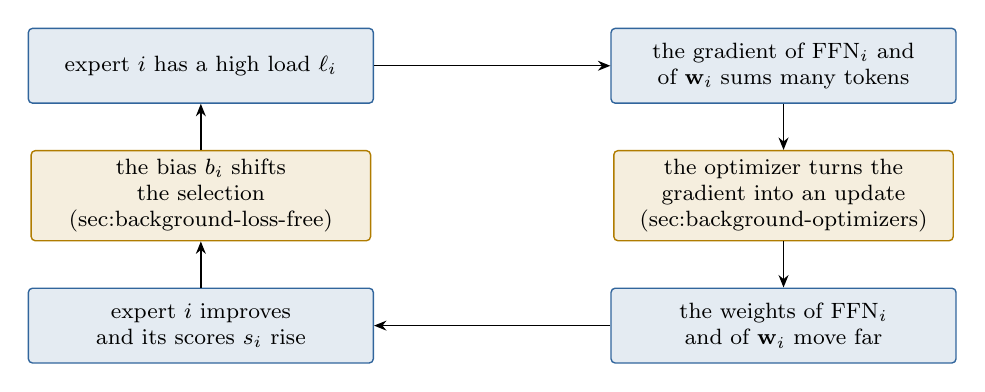
\begin{tikzpicture}[
    x=1cm, y=1cm, font=\footnotesize, line width=0.5pt,
    >={Stealth[length=4.5pt, width=3.6pt]},
    stage/.style={draw=moeblue, fill=moeblue!13, rounded corners=1.5pt, align=center, inner sep=4pt, minimum height=0.95cm, text width=4.1cm},
    op/.style={draw=moeamber, fill=moeamber!13, rounded corners=1.5pt, align=center, inner sep=3pt, text width=4.1cm},
  ]
  \node[stage] (load) at (0, 3.3) {expert $i$ has a high load $\ell_i$};
  \node[stage] (grad) at (7.4, 3.3) {the gradient of $\operatorname{FFN}_i$ and of $\mathbf{w}_i$ sums many tokens};
  \node[stage] (update) at (7.4, 0) {the weights of $\operatorname{FFN}_i$ and of $\mathbf{w}_i$ move far};
  \node[stage] (score) at (0, 0) {expert $i$ improves and its scores $s_i$ rise};
  % The two interventions sit on the edges they act on.
  \node[op] (optim) at (7.4, 1.65) {the optimizer turns the gradient into an update (\cref{sec:background-optimizers})};
  \node[op] (bias) at (0, 1.65) {the bias $b_i$ shifts\\the selection (\cref{sec:background-loss-free})};
  \draw[->] (load) -- (grad);
  \draw[->] (grad) -- (optim);
  \draw[->] (optim) -- (update);
  \draw[->] (update) -- (score);
  \draw[->] (score) -- (bias);
  \draw[->] (bias) -- (load);
\end{tikzpicture}

\end{figure}

\subsection{Auxiliary-Loss and Auxiliary-Loss-Free Balancing}
\label{sec:background-loss-free}
The usual balancer has been an \emph{auxiliary loss} that penalizes uneven loads and is added to the training loss \cite{shazeer2017outrageously, lepikhin2021gshard, fedus2022switch}. In the form of the Switch Transformer, written in our notation, it is
\begin{equation}[eq:aux-loss]{}
  \mathcal{L}_{\mathrm{bal}} = \alpha E \sum_{i=1}^{E} \ell_i \bar{s}_i, \qquad \bar{s}_i = \frac{1}{N} \sum_{t=1}^{N} s_i(\mathbf{x}_t),
\end{equation}
where $\alpha$ is a coefficient and $\bar{s}_i$ is the mean score of expert $i$ over the batch. The loads are not differentiable, so the gradient flows only through the mean scores. The derivative of the loss with respect to $\bar{s}_i$ is $\alpha E \ell_i$, so gradient descent pushes down the score of each expert in proportion to its load. In this loss, the scores of a token are normalized to sum to one. The Switch Transformer computes them with a softmax, and DeepSeek-V3, whose router uses the sigmoid like ours, divides them by their sum. The scores therefore cannot all fall: what the busiest experts lose, the experts with lower loads gain, and these are then selected more often. The gradient reaches the router and, through the input of the router, the layers below it. In the experiments of Wang et~al.~\cite{wang2024lossfree}, a small $\alpha$ let the routing collapse, while an $\alpha$ large enough to balance the loads made the perplexity worse. They therefore call this gradient an interference gradient.

\emph{Loss-free balancing} \cite{wang2024lossfree} removes the auxiliary loss and balances the loads with the bias of \cref{eq:moe-selection}. The bias starts at zero. After every training step, the bias of each expert moves by a fixed amount $u$, called the \emph{update rate}, in the direction that corrects its load on the batch of that step,
\begin{equation}[eq:bias-update]{}
  b_i \leftarrow b_i + u \operatorname{sign}\Bigl( \frac{1}{E} - \ell_i \Bigr), \qquad i = 1, \dots, E.
\end{equation}
The bias of an expert that received more than its fair share decreases, so the expert is selected for fewer tokens in the following steps. The bias of an expert that received less increases. Each step changes a bias by the same amount, no matter how far the load of its expert is from the fair share. Unlike the auxiliary loss, the bias adds no term to the loss and receives no gradient.

Kimi K3, GLM-5.3, and DeepSeek-V4 select their experts with such a bias \cite{kimi2026k3, zai2026glm53, deepseek2026v4}. DeepSeek-V4 applies \cref{eq:bias-update} with $u = 0.001$. Like DeepSeek-V3, it also adds a loss of the form of \cref{eq:aux-loss}, with $\alpha = 10^{-4}$, to prevent extreme imbalance within each sequence \cite{deepseek2024v3, deepseek2026v4}. We call such a loss, added to the bias, the \emph{balance loss}.

\subsection{The Span of the Bias}
\label{sec:background-span}
When the bias is active, the loads say little about the router, because the bias keeps them close to the fair share, whichever experts the router prefers. In the experiments of Wang et~al.~\cite{wang2024lossfree}, for example, the busiest expert of a layer exceeds the fair share by only 4\% on average. What differs between two models is how much bias was needed. If the scores alone distribute the tokens evenly, the load of each expert falls above and below the fair share in turn, and every bias stays close to zero. If instead the scores consistently favor some experts, the biases of these experts decrease step after step, and those of the neglected experts increase. We summarize the bias of a layer by its \emph{span},
\begin{equation}[eq:bias-span]{}
  \operatorname{span}(\mathbf{b}) = \max_{i} b_i - \min_{i} b_i,
\end{equation}
and read it as the \emph{work} of the bias, that is, how far the bias has to shift the preferences of the router to keep the loads even. For example, suppose that the router gives one expert a score 0.1 higher than another for every token. The two then share the tokens only when the bias of the first is about 0.1 below that of the second, so the span is at least 0.1. Adding the same constant to every bias does not change the selection, so only the differences between the biases matter, and the span is the largest of them.

Since the scores lie in $(0, 1)$, the span has a ceiling. If $b_i - b_j \geq 1$ for two experts $i$ and $j$, then $s_i + b_i > s_j + b_j$ for every token, since $s_j - s_i < 1$. Expert $i$ then ranks above expert $j$ for every token. A token goes to its $k$ highest-ranked experts, so every token sent to $j$ is also sent to $i$, and $\ell_i \geq \ell_j$. \Cref{eq:bias-update} therefore cannot raise $b_i$ relative to $b_j$. A difference can thus grow only while it is below one, and by at most $2u$ in one step, so the span never exceeds $1 + 2u$. A span close to one means that, for nearly every token, the bias alone decides which of the experts with the highest and the lowest bias ranks higher.

\subsection{A Shared Direction in the Inputs of the Router}
\label{sec:background-offset}
An analysis of the inputs of the router by Wang et~al.~\cite{wang2026myth} bears directly on the bias. Let $\mathbf{x}_1, \dots, \mathbf{x}_N$ denote the inputs of the router for the $N$ tokens of a batch, and let $\mathbf{c}$ be their mean. The logit of expert $i$ for token $t$ splits as
\begin{equation}[eq:background-offset]{}
  \mathbf{w}_i^{\top} \mathbf{x}_t = \mathbf{w}_i^{\top} \mathbf{c} + \mathbf{w}_i^{\top} (\mathbf{x}_t - \mathbf{c}), \qquad \mathbf{c} = \frac{1}{N} \sum_{t=1}^{N} \mathbf{x}_t,
\end{equation}
where the first term is the same for every token. When the inputs share a direction, $\mathbf{c}$ is long compared with the deviations $\mathbf{x}_t - \mathbf{c}$. The first term then gives the logit of each expert an \emph{offset} that every token shares, and the offset passes into the scores of \cref{eq:moe-score}. When the offsets differ across the experts, every token prefers the experts with the largest ones. The bias then has to cancel these differences, as in the example of \cref{sec:background-span}, and its span grows. The authors argue that an auxiliary loss teaches the router to suppress such a shared direction (their Proposition~2). They also report that the routers of two models balanced by the bias alone, both trained with Muon, do not suppress it (their Section~4.1). They do not isolate the effect of the optimizer.

\section{AdamW and Muon}
\label{sec:background-optimizers}
Throughout this section, $\mathbf{W} \in \mathbb{R}^{p \times q}$ is one weight matrix of the model, and $\mathbf{W}_t$ is its value after training step $t$. The gradient of the loss with respect to it at step $t$ is $\mathbf{G}_t$, and the learning rate of that step is $\eta_t$. The two optimizers that we compare share two refinements of gradient descent. First, both use \emph{momentum}, a running average of past gradients that smooths the noise of the gradient. Second, both normalize the size of the update, AdamW entry by entry and Muon for each matrix as a whole.

\subsection{Coordinate-Wise Updates: AdamW}
\label{sec:background-adamw}
Adam \cite{kingma2015adam} treats the entries of a weight matrix like any other parameters. We therefore write its update for the vector $\boldsymbol{\theta}$ of the parameters that it trains, with gradient $\mathbf{g}_t$ at step $t$. It keeps exponential moving averages $\mathbf{m}_t$ and $\mathbf{v}_t$ of the gradient and of its elementwise square. AdamW \cite{loshchilov2019decoupled} adds a weight decay that is not divided by $\sqrt{\hat{\mathbf{v}}_t}$, so that it shrinks every parameter by the same factor,
\begin{equation}[eq:adamw-update]{}
  \begin{aligned}
    \mathbf{m}_t          & = \beta_1 \mathbf{m}_{t-1} + (1 - \beta_1) \, \mathbf{g}_t, \qquad \mathbf{v}_t = \beta_2 \mathbf{v}_{t-1} + (1 - \beta_2) \, \mathbf{g}_t \odot \mathbf{g}_t, \\
    \boldsymbol{\theta}_t & = \boldsymbol{\theta}_{t-1} - \eta_t \biggl( \frac{\hat{\mathbf{m}}_t}{\sqrt{\hat{\mathbf{v}}_t} + \epsilon} + \lambda \boldsymbol{\theta}_{t-1} \biggr).
  \end{aligned}
\end{equation}
Here $\mathbf{m}_0 = \mathbf{v}_0 = \mathbf{0}$, $\beta_1, \beta_2 \in [0, 1)$ are decay rates, and $\hat{\mathbf{m}}_t = \mathbf{m}_t / (1 - \beta_1^t)$ and $\hat{\mathbf{v}}_t = \mathbf{v}_t / (1 - \beta_2^t)$ correct the averages, which start at zero and are too small in the first steps. The division and the square root are taken elementwise, $\epsilon$ is a small constant that prevents division by zero, and $\lambda$ is the weight decay.

Two properties of this update matter for the comparison with Muon. First, it is coordinate-wise, that is, the update of a parameter depends only on the past gradients of that same parameter. Second, when $\epsilon$ is neglected, the size of the update is set by how consistent the gradient of the parameter has been and not by its scale. Multiplying all the gradients by a positive constant multiplies $\hat{\mathbf{m}}_t$ and $\sqrt{\hat{\mathbf{v}}_t}$ by the same constant, so their ratio does not change. This ratio is close to $\pm 1$ when the recent gradients of a parameter are nearly the same, so the parameter moves by about $\eta_t$. When the gradients fluctuate around zero, the ratio is close to zero and the parameter hardly moves.

\subsection{Orthogonalized Updates: Muon}
\label{sec:background-muon}
Muon \cite{jordan2024muon} accumulates the gradients of a weight matrix in a momentum matrix and \emph{orthogonalizes} the result before using it as the update. Every matrix $\mathbf{A} \in \mathbb{R}^{p \times q}$ of rank $r$ has a singular value decomposition $\mathbf{A} = \mathbf{U} \mathbf{S} \mathbf{V}^{\top}$. Here $\mathbf{U} \in \mathbb{R}^{p \times r}$ and $\mathbf{V} \in \mathbb{R}^{q \times r}$ have orthonormal columns, and $\mathbf{S}$ is the diagonal matrix of the $r$ positive singular values. The matrix maps the $j$-th column of $\mathbf{V}$ to the $j$-th column of $\mathbf{U}$ times the $j$-th singular value. The singular values therefore say how strongly the matrix acts along each of $r$ perpendicular directions. The orthogonalization of $\mathbf{A}$ is
\begin{equation}[eq:ortho]{}
  \operatorname{Ortho}(\mathbf{A}) = \mathbf{U} \mathbf{V}^{\top},
\end{equation}
which is $\mathbf{A}$ with every singular value replaced by one. It keeps the directions of $\mathbf{A}$ but acts equally along each of them. Our update of Muon follows Liu et~al.~\cite{liu2025moonlight}, with a momentum coefficient $\mu$:
\begin{equation}[eq:muon-update]{}
  \begin{aligned}
    \mathbf{M}_t & = \mu \mathbf{M}_{t-1} + \mathbf{G}_t,                                                                                    \\
    \mathbf{O}_t & = \operatorname{Ortho}(\mu \mathbf{M}_t + \mathbf{G}_t),                                                                  \\
    \mathbf{W}_t & = \mathbf{W}_{t-1} - \eta_t \bigl( 0.2 \sqrt{\max(p, q)} \; \mathbf{O}_t + \lambda \mathbf{W}_{t-1} \bigr),
  \end{aligned}
\end{equation}
with $\mathbf{M}_0 = \mathbf{0}$. The term $\mu \mathbf{M}_t + \mathbf{G}_t$ is the Nesterov form of the momentum, which gives the latest gradient more weight than $\mathbf{M}_t$ alone does. Liu et~al.\ added the weight decay and the factor $0.2 \sqrt{\max(p, q)}$ when they scaled Muon up to an MoE model with 16B parameters. The factor gives the entries of the update a root mean square of 0.2, in the range of a typical update of AdamW, so that the learning rate of AdamW can be reused. We nevertheless tune each optimizer separately (\cref{sec:method-tuning}).

Since a singular value decomposition at every step would be too slow, Muon approximates \cref{eq:ortho} with a few steps of a Newton--Schulz iteration. Our five steps use only matrix multiplications and leave the singular values between about 0.7 and 1.2 (\cref{app:configuration-optimizer}). As Jordan et~al.\ recommend, and like Liu et~al.\ and DeepSeek-V4, we train the embedding table and the output head with AdamW.

\subsection{What Orthogonalization Does to a Matrix Update}
\label{sec:background-orthogonalization}
Two norms measure the size of a matrix. The spectral norm $\lVert \mathbf{A} \rVert_2$ is its largest singular value, which is the most that the matrix can stretch a vector. The Frobenius norm $\lVert \mathbf{A} \rVert_{\mathrm{F}}$ is the square root of the sum of its squared entries, which equals the square root of the sum of its squared singular values. All the singular values of $\mathbf{O}_t$ equal one, so $\lVert \mathbf{O}_t \rVert_2 = 1$ and $\lVert \mathbf{O}_t \rVert_{\mathrm{F}} = \sqrt{r}$. By \cref{eq:muon-update}, the spectral norm of a step of Muon, apart from the weight decay, is therefore $0.2 \, \eta_t \sqrt{\max(p, q)}$. It is set by the learning rate and the shape of the matrix, and it does not depend on the gradients.

The first consequence concerns the routed experts. The gradient of a matrix of an expert is a sum with one term for each token routed to the expert, so it tends to be larger for an expert with a high load \cite{wang2026depth}. AdamW removes the scale of the gradient but not its noise. The gradient of an expert with a low load is a sum over few tokens, so it varies more from one step to the next. By the second property of \cref{sec:background-adamw}, such an expert can therefore be expected to move less. Under Muon, the update of every expert matrix has the same spectral norm for any load of the expert. It also has nearly the same Frobenius norm, $\sqrt{r}$ times the spectral norm. In our runs, the gradient of an expert with the fair share is a sum of 8,192 terms of rank one, one per token, which gives it the full rank $r = \min(p, q)$. We therefore expected the updates of Muon to weaken the feedback of \cref{fig:background-feedback} (\cref{sec:results-rq1}).

The second consequence concerns the router $\mathbf{W}_{\mathrm{r}} \in \mathbb{R}^{E \times d}$, which has fewer rows than columns, with $E = 32$ and $d \geq 512$ in our models. If the matrix that is orthogonalized has rank $E$, then $\mathbf{U}$ is a square orthogonal matrix, so $\mathbf{O}_t \mathbf{O}_t^{\top} = \mathbf{U} \mathbf{V}^{\top} \mathbf{V} \mathbf{U}^{\top} = \mathbf{U} \mathbf{U}^{\top} = \mathbf{I}$. That is, the rows of the update are orthonormal. Wang et~al.~\cite{wang2026depth} show this property for the router of an MoE layer, in which row $i$ determines only the score of expert $i$. The update therefore moves the row of every expert by the same distance, $0.2 \, \eta_t \sqrt{d}$, no matter how much the gradients of the rows differ in size. Under AdamW, by contrast, the update of a row depends only on its own gradient, which comes only from the tokens that select its expert. Wang et~al.\ stress that this balances the updates of the rows, not directly the loads.

\section{Training Instability}
\label{sec:background-instability}
Two kinds of instability are reported in training large language models: divergences and loss spikes. In a \emph{divergence}, the loss grows until it is no longer finite or until the model is no better than at initialization. A \emph{loss spike} is a sharp increase of the training loss within a few steps, after which the loss usually returns to its previous level. Spikes appear in large models even when the gradient is clipped, that is, rescaled whenever its norm exceeds a threshold \cite{chowdhery2023palm, pascanu2013difficulty}. The router z-loss of Zoph et~al.~\cite{zoph2022stmoe} stabilizes MoE models by penalizing large router logits, which cause rounding errors in a router that normalizes them with a softmax. The DeepSeek-V4 report links the loss spikes of its training to \emph{outliers} in the MoE layers, that is, to very large activations. It adds that the routing appears to make these outliers larger \cite{deepseek2026v4}.

% !TEX root = ../main.tex
\chapter{Related Work}
\label{sec:related-work}

We call the set of choices with which a model is trained, such as its optimizers and its balancer, its \emph{recipe}. \Cref{sec:related-router} reviews which optimizer current recipes use for the router. \Cref{sec:related-muon-balance} reviews how Muon affects the balance of the experts, and \cref{sec:related-balancer} reviews the loss-free balancer. \Cref{sec:related-stress} reviews how high learning rates are used to study instability in small models.

\section{Where Training Recipes Put the Router}
\label{sec:related-router}
Most reports of current frontier models state which parameters Muon trains. Only one of them says why the router is or is not on Muon, and none show data that compare the options (\cref{tab:related-router}). DeepSeek-V4 excludes from Muon only the embedding table, the output head, the gains of the normalization layers, and a few small parameters \cite{deepseek2026v4}. Kimi K3 states that Muon trains its weight matrices and lists no exception \cite{kimi2026k3}. The router of both models is therefore on Muon, although neither report names it. GLM-5.3 refers to the GLM-5 report, which does not state the optimizer of the router \cite{glm2026glm5, zai2026glm53}.

\begin{table}[Where training recipes put the router]{tab:related-router}{Where current frontier models put the router. In the Router column, Muon means that the report does not exclude the router from Muon. The balancer is as stated in the report or the released configuration. The last column summarizes what the report says about the router or the balance.}
  \small
  \begin{tabular}{@{}lll>{\raggedright\arraybackslash}p{8.6cm}@{}}
    \toprule
    Model               & Router     & Balancer                  & What the report says                                                             \\
    \midrule
    DeepSeek-V4         & Muon       & bias, balance loss        & loss spikes occurred with outliers in the MoE layers                             \\
    Kimi K3             & Muon       & bias from scores          & a fixed bias step adapts slowly or oscillates                                    \\
    GLM-5.3             & not stated & bias                      & nothing about the router                                                         \\
    Qwen3.8-Flash-Next  & AdamW      & not stated                & Muon made the router unstable early, with no clear gain later                    \\
    MiMo-V2.6           & AdamW      & not stated                & frozen in reinforcement learning after it unbalanced the loads                  \\
    \bottomrule
  \end{tabular}
\end{table}

Two recipes keep the router on AdamW\@. Qwen3.8-Flash-Next trains its attention and experts with Muon. It trains the router with AdamW, because Muon made the router unstable early in training and gave no clear gain later. As one possible explanation, its report notes that each output of the router is the score of one expert, largely independent of the others, so the orthogonalization has no shared structure to exploit \cite{qiu2026qwennext}. MiMo-V2.6 moved most of its weight matrices from AdamW to Muown, a variant of Muon \cite{lion2026muown}, in mid-training. Its router, embedding table, and output head stayed on AdamW, for no stated reason. During reinforcement learning, the router drifted until the busiest expert of a layer received 16 times its fair share, so it was frozen for that stage \cite{xiaomi2026mimov26}. The disagreement between the recipes therefore rests on no controlled experiment. Our research questions RQ2 and RQ3 (\cref{sec:introduction-objectives}) provide such an experiment at a small scale. At raised learning rates, RQ2 compares all parameters on AdamW, all on Muon, and all on Muon except the router. RQ3 moves each part of the network to Muon in turn.

\section{Muon and the Balance of the Experts}
\label{sec:related-muon-balance}
The study closest to this thesis is that of Wang et~al.~\cite{wang2026depth}. They show that at initialization, the balance of a router with random weights is bounded by how similar the normalized hidden states of different tokens are. They then train a 500M-parameter MoE model with 2 of 16 experts selected and no balancer at all, for 2,000 steps with one seed. Under Muon, the usage of the experts stays balanced and the loss is lower, while under AdamW the balance decays during training. Their analysis concerns the update of the router (\cref{sec:background-orthogonalization}), but their experiments change the optimizer of the whole model. Our partitions separate the two. The analysis of the shared direction in \cref{sec:background-offset} comes from their companion paper \cite{wang2026myth}. Li \cite{li2026spectralcap} reports a related effect in a 64-expert MoE model trained with Muon and the bias. In its first MoE layer, one direction carries 0.995 of the variance of the logits plus the bias. The study uses one seed and has no run with AdamW.

Two studies change the optimizer of the router alone. Lau and Su \cite{lau2026symmetry} derive update rules that respect the structure of the router. They train the attention and the experts with Muon-style updates, remove the auxiliary loss, and find that their rules reach a lower validation loss than AdamW on the router. With and without the auxiliary loss, their rules also make the loads more even. None of their runs use the bias. Srivastava \cite{srivastava2026lossfree} trains the router with Adam or with Muon in a 1.47B-parameter model that selects 2 of 64 experts. Muon trains the attention and the experts in every run, and one of three balancers, the bias among them, keeps the loads even. Under Muon, the router is better conditioned, that is, its largest and smallest singular values are closer together, and the loss is nearly the same.

A study of another optimizer reports the balance as a side result. In an 8B-parameter model balanced by the bias, the busiest expert exceeds its fair share more under AdamW than under Muon \cite{xie2026spectralsphere}.

None of the studies above measure the work of the balancer, vary the optimizer of the backbone apart from that of the router, or measure the inputs of the router under each optimizer.

\section{The Loss-Free Balancer}
\label{sec:related-balancer}
The paper that introduced the bias tried three update rates for \cref{eq:bias-update}. A rate of $10^{-4}$ balanced the loads poorly early in training, and one of $10^{-2}$ made the balance worse late in training. The authors kept $10^{-3}$, which DeepSeek-V3 and Moonlight also use \cite{wang2024lossfree, deepseek2024v3, liu2025moonlight}. Two recipes trained with Muon replaced this fixed step. Trinity Large damps it, because near balance the rule oscillates \cite{singh2026trinity}. Kimi K3 sets every bias directly from the scores of the batch, since a fixed step either adapts slowly or makes the loads oscillate \cite{kimi2026k3}. Han and Zhong \cite{han2025lossfree} prove that the rule approximately balances the loads, and the optimizer plays no role in their analysis.

Several reports find the lowest MoE layers the hardest to balance. In OLMoE, the routing of the first layer settles much later than that of the others, and the authors note that this may impair the balance \cite{muennighoff2025olmoe}. Sigma-MoE-Tiny, trained with AdamW, selects one of 96 experts. In preliminary runs with the loss-free balancer, the bias of its lower layers grew until it decided the routing, and one expert received about 40 times its fair share \cite{hu2025sigmamoe}. Motif 3 was trained with Muon. It gave the balance loss of its first MoE layers a larger coefficient, because they were the most unbalanced early in training. Their routing still collapsed occasionally \cite{motif2026motif3}. None of these reports compare optimizers.

\section{Learning-Rate Stress Tests}
\label{sec:related-stress}
\label{sec:related-sensitivity}
\label{sec:related-stress-test}
Instabilities of large models are hard to study because small models with the same hyperparameters often do not show them. Wortsman et~al.~\cite{wortsman2024proxies} therefore reproduce divergences in small models trained at high learning rates, and they summarize the curve of the final loss against the learning rate in one number. Let $\mathcal{H}$ be a grid of learning rates, $\mathcal{L}_{\mathrm{val}}(\eta)$ the final validation loss of the model trained with the peak learning rate $\eta$, and $\mathcal{L}_{\mathrm{init}}$ the training loss at initialization. The \emph{learning-rate sensitivity} is
\begin{equation}[eq:lr-sensitivity]{}
  \operatorname{sens}(\mathcal{H}) = \frac{1}{\lvert \mathcal{H} \rvert} \sum_{\eta \in \mathcal{H}} \Bigl( \min \bigl( \mathcal{L}_{\mathrm{val}}(\eta), \, \mathcal{L}_{\mathrm{init}} \bigr) - \mathcal{L}^{*} \Bigr), \qquad \mathcal{L}^{*} = \min_{\eta \in \mathcal{H}} \mathcal{L}_{\mathrm{val}}(\eta),
\end{equation}
that is, the mean distance of the final loss from the best final loss of the grid. The minimum with $\mathcal{L}_{\mathrm{init}}$ counts a diverged run as a model that has learned nothing. A low sensitivity means that the loss changes little when the learning rate is far from its best value. Since the best rates of Muon and AdamW differ, we define each grid by multiples of the tuned rate of its optimizer, as the authors recommend.

The Qwen3.8-Flash-Next report \cite{qiu2026qwennext} uses high learning rates as a stress test. After the warmup, the learning rate is held at a multiple of its best value without decay, as in the long period that a production run spends near its peak learning rate. The report trains an MoE model with 25B parameters, of which 3B are active, with AdamW and with two configurations of Muon, each at two and at four times the best learning rate. At twice the best rate, the run with AdamW had 4.3 spikes per 10,000 steps and the two runs with Muon had 0.2, even though their activations were larger. At four times the best rate, the run with AdamW had 183. The report describes one run per configuration and does not measure the routing. Moreover, AdamW trains the router in the Muon runs of the report, so these runs leave open what the optimizer of the router contributes. RQ2 applies this stress test to three partitions, with three seeds and with the routing recorded (\cref{sec:results-rq2}).

% !TEX root = ../main.tex
\chapter{Method}
\label{sec:method}

We train one family of MoE language models many times on the same data and vary which optimizer, AdamW or Muon, trains each group of parameters. The bias of \cref{sec:background-loss-free} is the only balancer of our models, so the span of \cref{sec:background-span} measures all the work of balancing. The one exception is an experiment that adds a balance loss. This chapter describes what the experiments share and lists them in \cref{tab:method-program}. \Cref{app:configuration} gives every setting that this chapter leaves out.

\section{Data}
\label{sec:method-data}
We train on the sample-10BT subset of FineWeb-Edu \cite{penedo2024fineweb}, a corpus of educational web text. It is split into tokens by byte-level byte-pair encoding \cite{radford2019language} with a vocabulary of 16,384 symbols, which gives 10.07B training tokens. We hold out 1\% of the data for validation. A training sequence is a window of 1,025 consecutive tokens, in which each of the last 1,024 tokens is predicted from the tokens before it. A permutation fixed by the seed of the run shuffles the windows, so two runs with the same seed see the same tokens in the same order. The validation loss is the mean cross-entropy on 2.1M held-out tokens, the same in every run. It is measured every 250 steps and at the last step.

We measure the specialization of the experts (\cref{sec:method-readings}) on a panel of four domains with 2M tokens each: web text from a held-out shard of FineWeb-Edu, mathematics from OpenWebMath \cite{paster2024openwebmath}, source code from codeparrot-clean-valid \cite{codeparrot2022clean}, and articles from the English Wikipedia \cite{wikimedia2023wikipedia}.

\section{Models}
\label{sec:method-architecture}
Our models are the decoder-only Transformers of \cref{fig:background-model} \cite{vaswani2017attention, radford2019language}. Their attention uses rotary position embeddings, which encode the order of the tokens \cite{su2024roformer}. It also normalizes the queries and the keys of each head \cite{henry2020qknorm, dehghani2023vit22b}, and it multiplies its result by a gate before the output projection \cite{qiu2025gated}. Block 0 has a dense SwiGLU FFN\@. Every other block has the MoE layer of \cref{sec:background-moe}, with one shared expert and $E = 32$ routed experts, of which $k = 4$ are selected for each token.

After every optimizer step, the bias is updated by \cref{eq:bias-update} with $u = 0.001$, using the loads of the batch of that step. DeepSeek-V3 stops these updates toward the end of training \cite{deepseek2024v3}, but we keep them until the last step. We leave out the router z-loss (\cref{sec:background-instability}) and the changes that DeepSeek-V3 makes to the attention and to the training objective \cite{deepseek2024v3}.

We train models of two sizes, whose full settings are in \cref{tab:configuration-architecture}. The \emph{small} model has 8 blocks of width 512, with 8 attention heads and experts of hidden width 768. It has 303M parameters in total, of which 55M are active, that is, used for each token. The \emph{large} model has 12 blocks of width 768, with 12 heads and experts of hidden width 512. It has 496M parameters in total, of which 108M are active. The active counts leave out the embedding table and the output head, which the totals include. Both sizes have the same number of experts and the same $k$, a dense block 0, a context of 1,024 tokens, and a batch of 64 sequences. An expert with the fair share of the load receives $64 \times 1{,}024 \times k / E = 8{,}192$ tokens per step. We call the MoE layer of block 1 the \emph{first MoE layer}.

\section{Optimizers and Partitions}
\label{sec:method-optimizers}
We divide the parameters into six groups: the routers, the routed experts, the shared experts, the attention, the dense FFN of block 0, and a last group with the embedding table, the output head, and the gains of the normalization layers. The attention group holds the query, key, value, gate, and output projections. The last group is trained with AdamW in every run, as in the reports that use Muon (\cref{sec:background-muon}). We call an assignment of the optimizers to the other five groups a \emph{partition}. The four groups other than the routers form the backbone of \cref{sec:introduction-findings}, that is, every matrix of the model except the routers, the embedding table, and the output head.

\Cref{tab:method-partitions} lists the partitions that we use and the names by which we refer to them. The partitions AdamW and Muon train all five groups with one optimizer, and most others are named by what they train with Muon. The first three partitions are the choices of current models. DeepSeek-V3 trains all five groups with AdamW \cite{deepseek2024v3}, and DeepSeek-V4 \cite{deepseek2026v4} and Moonlight \cite{liu2025moonlight} train all five with Muon. Qwen3.8-Flash-Next trains its attention and experts with Muon but its router with AdamW \cite{qiu2026qwennext}. The next five partitions put Muon on one or two groups, and the last one is a control, described below.

\begin{table}[The partitions]{tab:method-partitions}{The partitions that we use. A partition trains with AdamW the groups that it does not put on Muon. The embedding table, the output head, and the gains are always trained with AdamW.}
  \small
  \begin{tabular}{lll}
    \toprule
    Partition                     & Groups trained with Muon                    & Used in                                     \\
    \midrule
    AdamW                         & none                                        & every experiment                            \\
    Muon                          & all five                                    & every experiment                            \\
    Muon, router on AdamW         & all but the router                          & RQ2, RQ3, balance loss, large model         \\
    Router on Muon                & the router                                  & RQ3                                         \\
    Experts on Muon               & the routed experts                          & RQ3                                         \\
    Attention on Muon             & the attention                               & RQ3                                         \\
    Dense FFN on Muon             & the dense FFN of block 0                    & RQ3                                         \\
    Attention, dense FFN on Muon  & the attention and the dense FFN             & RQ3                                         \\
    Control                       & all five, without the orthogonalization & tuning                                      \\
    \bottomrule
  \end{tabular}
\end{table}

Muon follows \cref{eq:muon-update} with $\mu = 0.95$, five Newton--Schulz steps, and $\lambda = 0.1$, as in Moonlight~\cite{liu2025moonlight}. AdamW follows \cref{eq:adamw-update} with $\beta_1 = 0.9$, $\beta_2 = 0.95$, and $\lambda = 0.1$, as in DeepSeek-V3 and DeepSeek-V4 \cite{deepseek2024v3, deepseek2026v4}. Muon treats the router of each MoE layer as one matrix. As in DeepSeek-V4 \cite{deepseek2026v4}, it treats each of the three matrices of every routed expert as a separate matrix.

The \emph{control} keeps the momentum of Muon and the size of its update, but not the orthogonalization. It rescales the Nesterov momentum $\mu \mathbf{M}_t + \mathbf{G}_t$ of each matrix to the Frobenius norm $\sqrt{\min(p, q)}$ of an orthogonal matrix of full rank. It then applies the factor $0.2 \sqrt{\max(p, q)}$ and the weight decay of \cref{eq:muon-update}. The updates of all the experts therefore have the same size, as under Muon, but the singular values of each update remain as unequal as those of the momentum (\cref{sec:background-orthogonalization}).

\section{Learning Rates, Schedule, and Clipping}
\label{sec:method-tuning}
The best learning rates of AdamW and Muon differ (\cref{sec:related-sensitivity}). Before any comparison, we therefore tune the peak learning rate of each optimizer separately, as benchmarks of optimizers do \cite{wen2025fantastic, semenov2025benchmarking}. We tune on the small model, with seed 0 and 0.5B tokens. We select the rate with the lowest validation loss at the end of the decay, since the loss curves of two optimizers can cross during it \cite{wen2025fantastic}. We try five rates for AdamW, five for Muon, and six for the control, each twice the one before (\cref{tab:configuration-optimizer}). Each optimizer is tuned on the partition that trains all five groups with it. In the runs of Muon and of the control, AdamW still trains the embedding table, the output head, and the gains, at the rate selected for AdamW\@. The tuned rates are $2 \times 10^{-3}$ for AdamW and $4 \times 10^{-3}$ for Muon. Every run of the small model uses them unless its design says otherwise.

The best learning rate changes with the width and falls as a run gets longer. For AdamW, Bjorck et~al.~\cite{bjorck2025horizons} find that it falls approximately as the number of tokens to the power $-0.32$, and so does that of a variant of Muon \cite{ren2026hypersphere}. Both fits come from larger models or longer runs than ours, and Bjorck et~al.\ find a steeper fall in their smallest models. We therefore tune the large model again, with 1B tokens and seed 0, at 0.125 to 1 times the rates of the small model. This tuning selected $10^{-3}$ for AdamW and $2 \times 10^{-3}$ for Muon. The runs of the large model use 3B tokens, three times as many as its tuning, so we multiply these rates by $3^{-0.32} \approx 0.7$. This gives $7 \times 10^{-4}$ for AdamW and $1.4 \times 10^{-3}$ for Muon.

The learning rate of each optimizer rises linearly from zero to its peak over a warmup of 500 steps. It then decays along a cosine to one tenth of the peak at the last step (\cref{eq:configuration-schedule}). The stress runs of RQ2 are the exception: after the warmup, they hold the rate at 1, 2, 4, 8, or 16 times the peak. The gradient is clipped separately for each optimizer, on the norm of the gradient of its own parameters. The threshold is 1.0. In the stress runs, it is instead twice the median gradient norm after the warmup of a calibration run, which trains the same partition at its tuned rates (\cref{tab:configuration-optimizer}).

\section{Measurements}
\label{sec:method-measurements}
Every 10 steps, a run writes a log. The log holds the training loss of every step since the previous log, the norm of the gradient of each optimizer before clipping, and the metrics of \cref{tab:method-readings} for every MoE layer. Most of these metrics are computed on the batch of that step, during the forward pass of training. The rest of this section defines them. At the same steps, the run copies the parameters before the optimizer step, so that it can measure the change that the step makes. Two runs that differed only in which metrics they computed had bit-identical losses, so computing them does not change the training.

\begin{table}[The metrics of a run]{tab:method-readings}{The metrics of a run, with what each says in words and its possible range in our models. Each metric is computed in one MoE layer or averaged over the MoE layers. The fair share of an expert is $1/E = 1/32$ of the routing slots.}
  \small
  \begin{tabular}{p{3.5cm}p{9.6cm}p{1.9cm}}
    \toprule
    Metric                   & What it says                                                                                          & Range                     \\
    \midrule
    Span                     & how far apart the biases are, that is, how hard the balancer works                   & 0 to $1 + 2u$             \\
    Input cosine             & how strongly the inputs of the router point in one shared direction                                   & 0 to 1                    \\
    Score offset             & how much more the router prefers some experts, equally for every token                        & 0 to 1                    \\
    Overload                 & the load of the busiest expert as a multiple of the fair share                                        & 1 (even) to 8             \\
    Usage perplexity         & the number of experts in even use                                                                      & 4 to 32 (even)            \\
    Load churn               & the smallest share of the slots that must change expert between logs                          & 0 to 1                    \\
    Specialization           & how differently the experts are used by text from four domains                                         & 0 to $\log 4$             \\
    Update--load correlation & whether experts that receive more tokens also receive larger updates                                   & $-1$ to 1                 \\
    Common share             & the share of the update of the router along the shared direction & 0 to 1 \\
    Largest activation       & the largest entry of the residual stream, the logits, or the expert outputs & from 0                    \\
    Spikes                   & the steps whose loss jumps well above that of the steps around them                          & a count                   \\
    \bottomrule
  \end{tabular}
\end{table}

\subsection{Windows}
\label{sec:method-windows}
A metric becomes one number per run by averaging it over the logged steps of a window, either in the first MoE layer or over all the MoE layers. The \emph{integrated} value is the mean from the end of the warmup to the end of the run, that is, over the logged steps $t$ with $500 < t \leq S$ in a run of $S$ steps. We report it unless we name another window. The \emph{early} value is the mean over the $0.05\,S$ steps that follow the warmup, which are steps 501 to 1,262 in a run of 1B tokens. The \emph{warmup} value is the mean over steps 1 to 500, and the \emph{final} value is the value at the last log. A difference between two biases changes by at most $2u$ per step (\cref{sec:background-span}). The span therefore takes hundreds of steps to respond to a change in the scores, so we measure it over such windows and not at single steps.

\subsection{Metrics of the Routing}
\label{sec:method-readings}
Besides the span of \cref{eq:bias-span}, two metrics describe the inputs of the router and the scores that it gives them. The \emph{input cosine} is the mean cosine similarity between the inputs of the router for two distinct tokens of the batch. With $\hat{\mathbf{x}}_t = \mathbf{x}_t / \lVert \mathbf{x}_t \rVert$, it is computed exactly from the sum of the $\hat{\mathbf{x}}_t$,
\begin{equation}[eq:method-cosine]{}
  \rho = \frac{1}{N (N - 1)} \sum_{t \neq t'} \hat{\mathbf{x}}_t^{\top} \hat{\mathbf{x}}_{t'} = \frac{\bigl\lVert \sum_{t=1}^{N} \hat{\mathbf{x}}_t \bigr\rVert^2 - N}{N (N - 1)}.
\end{equation}
It is close to the squared length of the mean of the normalized inputs. It therefore measures how strongly the inputs share the direction of \cref{sec:background-offset}: it is near zero when the inputs point in all directions, and one when they all point in the same direction. The \emph{score offset} is $\max_i \bar{s}_i - \min_i \bar{s}_i$, where $\bar{s}_i$ is the mean over the batch of the score $s_i$ of \cref{eq:moe-score}, not normalized. It is the spread of the offset of \cref{eq:background-offset} across the experts, as it appears in the scores. In other words, it is the preference for some experts that every token shares and that the bias has to cancel.

Three metrics describe the loads of \cref{eq:moe-load}. The \emph{overload} $E \max_i \ell_i$ is the load of the busiest expert divided by the fair share. It is 1 when the loads are even, and $E / k = 8$ when the same $k$ experts receive every token. The \emph{usage perplexity} of Wang et~al.~\cite{wang2026depth} is the exponential of the entropy of the loads, $\exp(-\sum_i \ell_i \log \ell_i)$. It is the number of experts in even use, from 32 when the loads are even down to 4 in the same extreme. The \emph{load churn}, related to the routing fluctuation of StableMoE \cite{dai2022stablemoe}, is the total variation distance $\frac{1}{2} \sum_i \lvert \ell_i - \ell_i' \rvert$ between the loads $\boldsymbol{\ell}$ of a log and the loads $\boldsymbol{\ell}'$ of the previous log. It is the smallest fraction of the routing slots that would have to change expert to turn one distribution of the load into the other.

The \emph{specialization} is measured on the panel of \cref{sec:method-data} at the last checkpoint. Following Muennighoff et~al.~\cite{muennighoff2025olmoe}, we compute the loads of \cref{eq:moe-load} over the tokens of each domain. We then summarize the four distributions of a layer by their Jensen--Shannon divergence, that is, the entropy of their mean minus the mean of their entropies. It is zero when the domains are routed alike and $\log 4$ when no two domains share an expert. The \emph{update--load correlation} is computed across the 32 routed experts of a layer. It is the Pearson correlation between the number of tokens routed to an expert in a step and the size of the change that the step makes to the expert. We measure this size by the Frobenius norm of the three matrices of the expert, taken as one. We also report the same correlation for the largest spectral norm of the three matrices, which is the size that Muon fixes (\cref{sec:background-orthogonalization}).

The \emph{common share} measures how much of the update of the router acts on the shared direction of its inputs. Let $\Delta \mathbf{W}_{\mathrm{r}}$ denote the change that a step makes to the router, and let $\hat{\mathbf{c}}$ be the unit vector along $\sum_t \hat{\mathbf{x}}_t$. Since the normalization gives the inputs similar lengths, $\hat{\mathbf{c}}$ is close to the direction of the mean input $\mathbf{c}$ of \cref{eq:background-offset}. The common share is
\begin{equation}[eq:method-common-share]{}
  \kappa = \frac{\lVert \Delta \mathbf{W}_{\mathrm{r}} \, \hat{\mathbf{c}} \rVert}{\lVert \Delta \mathbf{W}_{\mathrm{r}} \rVert_{\mathrm{F}}},
\end{equation}
where the numerator is the change that the step makes to the logits of the experts for the direction $\hat{\mathbf{c}}$. The common share is one when the update moves every row of the router along $\hat{\mathbf{c}}$ only. For an update whose $E$ singular values are equal, the numerator is at most the spectral norm, and the denominator is $\sqrt{E}$ times the spectral norm. The common share of such an update is therefore at most $1 / \sqrt{32} \approx 0.18$. The update of Muon is close to this case, since the Newton--Schulz steps leave its singular values near one (\cref{sec:background-muon}) and the weight decay adds a small term. The update of AdamW has no such bound.

\subsection{Metrics of Stability}
\label{sec:method-stability}
Every log also records, in every block, the largest absolute entry of the residual stream, of the attention logits (the dot products of the queries with the keys), of the router logits, and of the outputs of the routed experts. A step is a \emph{spike} if the excess of its training loss over the median of the 201 steps centered on it is above two thresholds. The first is 0.1, the threshold of the Qwen3.8-Flash-Next report \cite{qiu2026qwennext}. The second is five robust standard deviations of the excess in the same window, estimated from the median absolute deviation, as in the K2-V2 report \cite{k2team2025k2v2}. With our batch, this standard deviation is about 0.04, so the first threshold alone would flag the ordinary fluctuation of the loss. The second alone would flag negligible excesses where the loss is very smooth. Spikes on consecutive steps form one \emph{episode}. A run has \emph{diverged} when its training loss or a gradient norm stops being finite, or when its final validation loss is at or above its initial training loss. We compute the learning-rate sensitivity of a partition by \cref{eq:lr-sensitivity} over its stress runs at 1 to 8 times its tuned rates. There, $\mathcal{L}_{\mathrm{init}}$ is the initial training loss, and the final losses are averaged over the seeds.

\section{Experiments}
\label{sec:method-experiments}
\Cref{tab:method-program} lists the experiments. Each experiment compares a few configurations, which we call its \emph{arms}, and \cref{app:configuration-program} lists them. Most arms are partitions, and some change one more setting. Muon at half rate trains with half the tuned rate of Muon, that is, at the rate of AdamW\@. AdamW and Muon without the bias hold the bias at zero, so that nothing balances the loads. The fast bias moves by $4u = 0.004$ per step instead of $u = 0.001$. The balance-loss experiment adds the balance loss of DeepSeek-V3 (\cref{sec:results-balance-loss}). No comparison is tested on the runs that suggested it. Every experiment designed from earlier results therefore trains new runs, with new seeds on the small model. The one exception is the balance-loss experiment, whose arms without the loss are the runs of RQ3.

\begin{table}[The experiments]{tab:method-program}{The experiments. Every arm is trained at each seed of its row. The tuning trains one run per rate, and RQ2 adds one calibration run per partition. The 30 exploratory runs are not counted.}
  \small
  \setlength{\tabcolsep}{4pt}
  \begin{tabular}{@{}lll>{\raggedright\arraybackslash}p{9cm}rl@{}}
    \toprule
    Experiment    & Model & Tokens & Arms                                                   & Runs & Section                        \\
    \midrule
    Tuning        & small & 0.5B   & AdamW, Muon, control, over their rates; AdamW with $\beta_2 = 0.98$; seed 0 & 17   & \labelcref{sec:method-tuning}  \\
    RQ1           & small & 1B     & AdamW, Muon; seeds 0--2                                & 6    & \labelcref{sec:results-rq1}    \\
    RQ2, stress   & small & 0.5B   & AdamW, Muon, Muon with the router on AdamW, at five multiples; Muon with the fast bias at multiple 4; seeds 0--2 & 51 & \labelcref{sec:results-rq2}    \\
    RQ3           & small & 1B     & every partition but the control, Muon at half rate, AdamW and Muon without the bias; seeds 3--5 & 33 & \labelcref{sec:results-rq3} \\
    Bias speed    & small & 1B     & AdamW, Muon, with the usual and the fast bias; seeds 6--8 & 12 & \labelcref{sec:results-bias-speed} \\
    Balance loss  & small & 1B     & AdamW, Muon, Muon with the router on AdamW, with the balance loss; seeds 3--5 & 9 & \labelcref{sec:results-balance-loss} \\
    Tuning, large & large & 1B     & AdamW, Muon, over their rates; seed 0                 & 8    & \labelcref{sec:method-tuning}  \\
    Large model   & large & 3B     & AdamW, Muon, Muon with the router on AdamW; seeds 0--2                 & 9    & \labelcref{sec:results-large}  \\
    \midrule
    Total         &       &        &                                                        & 145  &                                \\
    \bottomrule
  \end{tabular}
\end{table}

We also report three sets of shorter runs as exploratory: eight runs that came before RQ3, and two probes. The eight runs, one for each partition of RQ3, used seed 0 and up to 0.5B tokens, and they suggested the design of RQ3. The two probes repeat the first 3,000 steps of runs of RQ3 and of the large model, most of them with one change. One such change subtracts the mean input of the batch from the input of the first router (Sections~\ref{sec:results-offset} and~\ref{sec:results-large}). A probe run without a change reproduces its full run bit for bit, so a changed run differs from its full run by the change alone.

\section{Comparisons}
\label{sec:method-statistics}
Every comparison is paired by seed. Its unit is the difference $\delta$ between the values of two runs with the same seed. We report the mean of $\delta$ over the seeds, followed in brackets by its range, from the smallest of the three differences to the largest. With three seeds, this range is also the 95\% percentile bootstrap interval \cite{efron1993introduction}. A resample of the three differences repeats the smallest one three times with probability $(1/3)^3 = 1/27$, which is above 2.5\%, and likewise the largest. This interval is narrower than a true 95\% interval \cite{agarwal2021precipice}, so we read it as the spread of the difference over the seeds rather than as a test. Two arms that do not differ give a difference with the same sign at every seed with probability $2 \times (1/2)^3 = 1/4$. Every run is reported.

We fixed the comparisons of each experiment, and the expected sign of each, before training its runs. \Cref{sec:results} notes the ones that went against what we expected. We apply no correction for the number of comparisons, and every unplanned analysis, including the probes, is exploratory.

A metric of the routing could differ between two runs merely because one of them is further along in training. We therefore also compute every planned difference at matched loss. To do so, we cut both runs of a pair at the first evaluation at which each reaches the worse of their two final validation losses. The two views led to the same conclusion for every planned difference, so we report the values at equal tokens. The specialization and the loss are compared at equal tokens only.

% !TEX root = ../main.tex
\chapter{Results}
\label{sec:results}

This chapter reports six experiments, one per section. \Crefrange{sec:results-rq1}{sec:results-rq3} answer the three research questions of \cref{sec:introduction-objectives}. The results of RQ3 led to two more experiments on the balancer. They test whether Muon still raises the span when the bias moves four times faster (\cref{sec:results-bias-speed}) and when we add the balance loss of DeepSeek-V3 (\cref{sec:results-balance-loss}). \Cref{sec:results-large} repeats the main comparisons on the large model.

Every section states its finding, describes the experiment, and reports the runs. The partitions have the names of \cref{tab:method-partitions}, and the value of an arm is its mean over the seeds. The tables give each difference between two arms, computed before rounding, with its range over the seeds (\cref{sec:method-statistics}).

\section{RQ1: Muon Against AdamW}
\label{sec:results-rq1}
At the tuned rates, the bias worked harder under Muon than under AdamW, mostly in the first MoE layer and early in training. This happened although Muon made the size of the update of an expert independent of its load.

RQ1 compares AdamW with Muon on the small model, with 1B tokens and seeds 0 to 2. Each optimizer trains at its tuned rate, $2 \times 10^{-3}$ for AdamW and $4 \times 10^{-3}$ for Muon. Under Muon, the update of an expert has the same size for any load (\cref{sec:background-orthogonalization}). We therefore expected no correlation between the size of the update and the load under Muon, unlike under AdamW\@. The feedback in which busy experts become busier (\cref{sec:background-feedback}) would then be weaker under Muon, so we expected a lower span and load churn.

\begin{table}[The results of RQ1]{tab:results-rq1}{The results of RQ1, on the small model with 1B tokens and seeds 0 to 2. Every metric is the integrated value averaged over the MoE layers, unless the row names another layer or window. The exceptions are the validation loss, taken at the last step, and the specialization, measured at the last checkpoint. The range is that of the three paired differences (\cref{sec:method-statistics}).}
  \begin{tabular}{lrrrl}
    \toprule
    Metric                            & AdamW   & Muon    & Difference  & Range                  \\
    \midrule
    Validation loss                   & 3.255   & 3.177   & $-0.078$    & [$-0.086$, $-0.062$]   \\
    Span                              & 0.105   & 0.137   & $+0.033$    & [$+0.030$, $+0.036$]   \\
    Span, first MoE layer             & 0.084   & 0.194   & $+0.110$    & [$+0.085$, $+0.151$]   \\
    Update--load correlation          & 0.379   & 0.024   & $-0.355$    & [$-0.362$, $-0.345$]   \\
    Update--load correlation, spectral norm & 0.102   & 0.035   & $-0.068$    & [$-0.073$, $-0.061$]   \\
    Load churn                        & 0.032   & 0.038   & $+0.006$    & [$+0.004$, $+0.008$]   \\
    Load churn, early                 & 0.049   & 0.064   & $+0.015$    & [$+0.011$, $+0.017$]   \\
    Load churn, warmup                & 0.102   & 0.083   & $-0.019$    & [$-0.020$, $-0.018$]   \\
    Specialization                    & 0.105   & 0.118   & $+0.014$    & [$+0.006$, $+0.017$]   \\
    \bottomrule
  \end{tabular}
\end{table}

The premise held: the update--load correlation was 0.38 under AdamW and 0.02 under Muon (\cref{tab:results-rq1}). The prediction did not. After the warmup, the span and the load churn were both higher under Muon, at every seed. The span was about a third higher, 0.137 against 0.105. It remained higher when the two runs of a pair were compared at matched loss, so the difference does not come from one model being further along in training. Muon also reached a lower validation loss and a higher specialization.

A higher span does not mean that the loads were less even. Outside the first MoE layer, the busiest expert received at most 1.3 times its fair share after the warmup, under both optimizers. In these layers, the bias kept the loads close to even, and the optimizers differed only in how far it had to move.

Most of the difference was in the first MoE layer (\cref{fig:results-rq1}). Its span was more than twice as large under Muon, whereas in the other six layers the difference was 0.02 on average. The difference was also largest early in training. Over steps 501 to 1,000, the span was 0.74 under Muon against 0.19 under AdamW\@. By the end of the run, it had fallen under both optimizers, but under Muon it was still about twice that of AdamW\@. We call this higher span of the first MoE layer the \emph{rise}.

\begin{figure}[The span under AdamW and Muon in RQ1 and in the tuning]{fig:results-rq1}{The span under AdamW and Muon. Left: the span of every MoE layer in RQ1, with the range over the seeds. Center: the span of the first MoE layer over training in RQ1, in bins of 100 steps. The range over the seeds is shaded, and the dashed lines are the mean span of the other six layers. Right: the span averaged over the layers in the tuning runs of AdamW, Muon, and the control, with 0.5B tokens and seed 0, against the peak learning rate. Filled marks are the selected rates.}
  % RQ1 in three panels: the span of every MoE layer under AdamW and Muon; the span of the first MoE layer over training, with the mean of the other six layers dashed; and the span over all the layers against the learning rate in the tuning. The data are figures/data/rq1-layers-*.csv, rq1-span-*.csv and tuning-*.csv.
\begin{tikzpicture}
  \begin{groupplot}[
      thesis,
      group style={group size=3 by 1, horizontal sep=1.45cm},
      width=4.05cm, height=3.3cm,
    ]
    \nextgroupplot[
      xlabel={MoE layer}, ylabel={Span},
      xtick={1,...,7}, xmin=0.5, xmax=7.5,
      ymin=0, ymax=0.25, ytick={0,0.05,0.1,0.15,0.2,0.25},
      yticklabel style={/pgf/number format/fixed, /pgf/number format/precision=2},
      legend pos=north east,
    ]
    \addplot[arm a, only marks, error bars/.cd, y dir=both, y explicit, error bar style={line width=0.5pt}]
      table[x expr=\thisrow{layer}-0.14, y=mean, y error plus expr=\thisrow{high}-\thisrow{mean}, y error minus expr=\thisrow{mean}-\thisrow{low}] {figures/data/rq1-layers-adamw.csv};
    \addlegendentry{AdamW}
    \addplot[arm b, only marks, error bars/.cd, y dir=both, y explicit, error bar style={line width=0.5pt}]
      table[x expr=\thisrow{layer}+0.14, y=mean, y error plus expr=\thisrow{high}-\thisrow{mean}, y error minus expr=\thisrow{mean}-\thisrow{low}] {figures/data/rq1-layers-muon.csv};
    \addlegendentry{Muon}

    \nextgroupplot[
      xlabel={Step (thousands)}, ylabel={Span},
      xmin=0, xmax=15.26, xtick={0,5,10,15},
      ymin=0, ymax=0.9, ytick={0,0.2,0.4,0.6,0.8},
      yticklabel style={/pgf/number format/fixed, /pgf/number format/precision=1},
    ]
    \addplot[name path=alo, draw=none, forget plot] table[x expr=\thisrow{step}/1000, y=first_low] {figures/data/rq1-span-adamw.csv};
    \addplot[name path=ahi, draw=none, forget plot] table[x expr=\thisrow{step}/1000, y=first_high] {figures/data/rq1-span-adamw.csv};
    \addplot[band, fill=moeamber, forget plot] fill between[of=alo and ahi];
    \addplot[name path=blo, draw=none, forget plot] table[x expr=\thisrow{step}/1000, y=first_low] {figures/data/rq1-span-muon.csv};
    \addplot[name path=bhi, draw=none, forget plot] table[x expr=\thisrow{step}/1000, y=first_high] {figures/data/rq1-span-muon.csv};
    \addplot[band, fill=moeblue, forget plot] fill between[of=blo and bhi];
    \addplot[moeamber, no marks] table[x expr=\thisrow{step}/1000, y=first] {figures/data/rq1-span-adamw.csv};
    \addplot[moeblue, no marks] table[x expr=\thisrow{step}/1000, y=first] {figures/data/rq1-span-muon.csv};
    \addplot[moeamber, no marks, dashed, line width=0.6pt] table[x expr=\thisrow{step}/1000, y=rest] {figures/data/rq1-span-adamw.csv};
    \addplot[moeblue, no marks, dashed, line width=0.6pt] table[x expr=\thisrow{step}/1000, y=rest] {figures/data/rq1-span-muon.csv};

    \nextgroupplot[
      xlabel={Learning rate ($\times 10^{-3}$)}, ylabel={Span},
      xmode=log, log basis x=2, xmin=1.6e-4, xmax=4.4e-2,
      xtick={2.5e-4,1e-3,4e-3,1.6e-2}, xticklabels={0.25, 1, 4, 16},
      xticklabel style={/pgf/number format/assume math mode=false},
      ymin=0, ymax=0.45, ytick={0,0.1,0.2,0.3,0.4},
      yticklabel style={/pgf/number format/fixed, /pgf/number format/precision=1},
      legend pos=north west,
    ]
    \addplot[arm a, mark options={fill=white}] table[x=rate, y=span] {figures/data/tuning-adamw.csv};
    \addlegendentry{AdamW}
    \addplot[arm b, mark options={fill=white}] table[x=rate, y=span] {figures/data/tuning-muon.csv};
    \addlegendentry{Muon}
    \addplot[arm f, mark options={fill=white}] table[x=rate, y=span] {figures/data/tuning-momentum.csv};
    \addlegendentry{Control}
    \addplot[arm a, only marks, forget plot] coordinates {(2e-3, 0.11256)};
    \addplot[arm b, only marks, forget plot] coordinates {(4e-3, 0.16235)};
    \addplot[arm f, only marks, forget plot] coordinates {(5e-4, 0.10688)};
  \end{groupplot}
\end{tikzpicture}

\end{figure}

The inputs of the first router also differed. In an exploratory analysis at the last checkpoint, on the panel of \cref{sec:method-data}, we measured a variant of the similarity that Wang et~al.\ use \cite{wang2026myth}: the mean cosine between the inputs of a router for two tokens of the same domain. In the first MoE layer, it was about 0.4 under Muon against 0.1 under AdamW, at every seed, so under Muon the inputs of the first router shared a direction. The difference shrank with depth, and in the last layer the cosine was lower under Muon, 0.21 against 0.26. By \cref{sec:background-offset}, a shared direction gives the scores an offset that the bias has to cancel. We designed RQ3 to find which part of the model produces this direction.

The tuning runs, which are exploratory, point to a second factor, the learning rate (\cref{fig:results-rq1}, right). In the tuning, the span grew with the rate under Muon but stayed flat under AdamW\@. Part of the rise may therefore come from the rate of Muon, which is twice that of AdamW, and RQ3 tests this. The control, Muon without the orthogonalization, also had a higher span than AdamW at every rate above its best (\cref{app:results-tuning}).

\section{RQ2: Learning-Rate Stress}
\label{sec:results-rq2}
Under learning-rate stress, no run diverged. The two Muon partitions reached the same loss, and at high multiples it exceeded that of AdamW\@. Contrary to what we expected from the Qwen3.8-Flash-Next report, the loads shifted more in the warmup with the router on AdamW than under Muon.

RQ2 applies the stress test of \cref{sec:related-stress-test} to AdamW, Muon, and Muon with the router on AdamW, the partition of the Qwen3.8-Flash-Next report \cite{qiu2026qwennext}. Each partition is trained with 0.5B tokens and seeds 0 to 2, at 1, 2, 4, 8, and 16 times its tuned rates, held constant after the warmup (\cref{sec:method-tuning}). Muon is also trained at four times its rates with the fast bias, which moves by $4u$ per step (\cref{sec:method-experiments}). Following the report, we expected the two Muon partitions to reach the same loss at every multiple, lower than that of AdamW\@. The report found that Muon made the router unstable early in training. We therefore also expected the loads to shift less during the warmup with the router on AdamW than under Muon. We measure this shift by the \emph{warmup churn}, the load churn of \cref{sec:method-readings} over the warmup.

\begin{figure}[The stress runs of RQ2]{fig:results-rq2}{The stress runs of RQ2 against the multiple of the tuned rates. The panels show the final validation loss, the load churn of the warmup averaged over the MoE layers, and the largest entries of the residual stream and of the router logits over the run. Lines join the means over the seeds, and in the last three panels the small marks are the seeds.}
  % RQ2 in four panels against the multiple of the tuned rates: the final validation loss, the load churn of the warmup over all the MoE layers, and the largest entries of the residual stream and of the router logits over the run. Lines join the means over the seeds and the small marks are the seeds. The data are figures/data/stress-*.csv.
\begin{tikzpicture}
  \begin{groupplot}[
      thesis,
      group style={group size=2 by 2, horizontal sep=1.7cm, vertical sep=1.25cm},
      width=6.3cm, height=3.0cm,
      xmode=log, log basis x=2, xmin=0.8, xmax=20,
      xtick={1,2,4,8,16}, xticklabels={1, 2, 4, 8, 16},
      xticklabel style={/pgf/number format/assume math mode=false},
    ]
    \nextgroupplot[
      ylabel={Final validation loss},
      ymin=3.5, ymax=4.5, ytick={3.6,3.8,4.0,4.2,4.4},
      yticklabel style={/pgf/number format/fixed, /pgf/number format/precision=1, /pgf/number format/fixed zerofill},
      legend pos=north west,
    ]
    \addplot[arm a] table[x=lr_multiplier, y=loss_capped] {figures/data/stress-adamw-mean.csv};
    \addlegendentry{AdamW}
    \addplot[arm b] table[x=lr_multiplier, y=loss_capped] {figures/data/stress-muon-mean.csv};
    \addlegendentry{Muon}
    \addplot[arm c] table[x=lr_multiplier, y=loss_capped] {figures/data/stress-muon_except_router-mean.csv};
    \addlegendentry{Muon, router on AdamW}

    \nextgroupplot[
      ylabel={Warmup churn},
      ymin=0.07, ymax=0.17, ytick={0.08,0.1,0.12,0.14,0.16},
      yticklabel style={/pgf/number format/fixed, /pgf/number format/precision=2, /pgf/number format/fixed zerofill},
    ]
    \addplot[arm a, only marks, mark size=0.7pt, forget plot] table[x=lr_multiplier, y=load_churn_warmup] {figures/data/stress-adamw.csv};
    \addplot[arm b, only marks, mark size=0.6pt, forget plot] table[x=lr_multiplier, y=load_churn_warmup] {figures/data/stress-muon.csv};
    \addplot[arm c, only marks, mark size=0.8pt, forget plot] table[x=lr_multiplier, y=load_churn_warmup] {figures/data/stress-muon_except_router.csv};
    \addplot[arm a] table[x=lr_multiplier, y=load_churn_warmup] {figures/data/stress-adamw-mean.csv};
    \addplot[arm b] table[x=lr_multiplier, y=load_churn_warmup] {figures/data/stress-muon-mean.csv};
    \addplot[arm c] table[x=lr_multiplier, y=load_churn_warmup] {figures/data/stress-muon_except_router-mean.csv};

    \nextgroupplot[
      xlabel={Multiple of the tuned rates}, ylabel={Largest residual entry},
      ymode=log, ymin=500, ymax=1e6,
    ]
    \addplot[arm a, only marks, mark size=0.7pt, forget plot] table[x=lr_multiplier, y=residual_max_peak] {figures/data/stress-adamw.csv};
    \addplot[arm b, only marks, mark size=0.6pt, forget plot] table[x=lr_multiplier, y=residual_max_peak] {figures/data/stress-muon.csv};
    \addplot[arm c, only marks, mark size=0.8pt, forget plot] table[x=lr_multiplier, y=residual_max_peak] {figures/data/stress-muon_except_router.csv};
    \addplot[arm a] table[x=lr_multiplier, y=residual_max_peak] {figures/data/stress-adamw-mean.csv};
    \addplot[arm b] table[x=lr_multiplier, y=residual_max_peak] {figures/data/stress-muon-mean.csv};
    \addplot[arm c] table[x=lr_multiplier, y=residual_max_peak] {figures/data/stress-muon_except_router-mean.csv};

    \nextgroupplot[
      xlabel={Multiple of the tuned rates}, ylabel={Largest router logit},
      ymode=log, ymin=10, ymax=300,
      ytick={10,30,100,300}, yticklabels={10, 30, 100, 300},
      yticklabel style={/pgf/number format/assume math mode=false},
    ]
    \addplot[arm a, only marks, mark size=0.7pt, forget plot] table[x=lr_multiplier, y=router_logit_max_peak] {figures/data/stress-adamw.csv};
    \addplot[arm b, only marks, mark size=0.6pt, forget plot] table[x=lr_multiplier, y=router_logit_max_peak] {figures/data/stress-muon.csv};
    \addplot[arm c, only marks, mark size=0.8pt, forget plot] table[x=lr_multiplier, y=router_logit_max_peak] {figures/data/stress-muon_except_router.csv};
    \addplot[arm a] table[x=lr_multiplier, y=router_logit_max_peak] {figures/data/stress-adamw-mean.csv};
    \addplot[arm b] table[x=lr_multiplier, y=router_logit_max_peak] {figures/data/stress-muon-mean.csv};
    \addplot[arm c] table[x=lr_multiplier, y=router_logit_max_peak] {figures/data/stress-muon_except_router-mean.csv};
  \end{groupplot}
\end{tikzpicture}

\end{figure}

No run diverged (\cref{fig:results-rq2}). At the tuned rates, the three partitions reached nearly the same loss. At higher multiples, the loss of AdamW rose less than that of the two Muon partitions. Over the multiples 1 to 8, the learning-rate sensitivity (\cref{eq:lr-sensitivity}) was 0.18 for AdamW and 0.24 for the Muon partitions. As expected, the losses of the two Muon partitions differed by at most 0.002 at every multiple.

The warmup churn went against what we expected. At every multiple, it was highest with the router on AdamW and lowest under Muon, and the ranges of these two partitions over the seeds did not overlap. With the fast bias, Muon at four times its rates reached the same loss as with the usual bias, and its warmup churn was lower. RQ3 found the same higher churn with the router on AdamW at the tuned rates, and \cref{sec:results-offset} traces it to how this router responds to the shared direction.

The largest activations grew with the rate under every partition. Up to four times the tuned rates, the largest entries of the residual stream under the Muon partitions were two to three times those of AdamW, as the report found. From eight times the tuned rates, those of AdamW grew faster. The largest activations therefore did not rank the partitions as the loss did. The largest router logits stayed below 36 at every multiple when AdamW trained the router, whereas under Muon they grew to 98 at 16 times the tuned rates. The 45 runs at the five multiples had seven episodes of loss spikes, six of them at 16 times the tuned rates. These are too few to relate to the routing (\cref{app:results-stress}).

\section{RQ3: Where the Rise Comes From}
\label{sec:results-rq3}
The optimizer of the router barely changed the span of the first MoE layer, whereas Muon on the backbone made it about twice as large. With Muon at the rate of AdamW, three quarters of this rise disappeared. Only the whole backbone on Muon gave the inputs of the first router a shared direction. Yet the routed experts alone on Muon raised the span the most, without as strong a direction.

RQ3 asks which group of parameters, trained with Muon, raises the span of the first MoE layer. The input of its router comes from the embedding table, the attention and the dense FFN of block 0, and the attention of block 1 (\cref{fig:background-model}). AdamW trains the embedding table in every partition. The routed experts affect this input only through the gradients that they send back to these layers.

Four partitions combine each optimizer of the router with each optimizer of the backbone: AdamW, the router alone on Muon, Muon with the router on AdamW, and Muon. Muon is also trained at half its rate, the rate of AdamW, to separate the optimizer from its larger rate. Four more partitions put Muon on one part of the backbone: the routed experts, the attention, the dense FFN, or the attention and the dense FFN together. Finally, AdamW and Muon are trained without the bias, and we call the other arms \emph{balanced}. Every arm is trained on the small model with 1B tokens and seeds 3 to 5. \Cref{fig:results-rq3} shows the balanced arms in three groups, which the next three subsections take in turn, and \cref{tab:results-rq3} gives their results. The \emph{early overload} is the early value of the overload (\cref{sec:method-windows}).

\begin{figure}[The first MoE layer in the balanced arms of RQ3]{fig:results-rq3}{The span, the input cosine, and the score offset of the first MoE layer in the balanced arms of RQ3, on the small model with 1B tokens. Dashed lines separate three groups: the four combinations of the optimizers of the router and of the backbone, Muon at half rate, and the four partitions with one part of the backbone on Muon. The bars are the means over seeds 3 to 5, and the marks are the seeds. The three arms with the whole backbone on Muon are in blue.}
  % RQ3: the span, the input cosine and the score offset of the first MoE layer for each balanced arm, one row per arm, in three groups split by dashed lines: the optimizers of the router and of the backbone crossed, Muon at half rate, and one part of the backbone on Muon. The bars are the means over seeds 3 to 5 and the marks are the seeds; blue marks the arms with the whole backbone on Muon. The data are figures/data/rq3-arms.csv and rq3-arms-mean.csv, which extract.py writes.
\begin{tikzpicture}
  \begin{groupplot}[
      thesis,
      group style={group size=3 by 1, horizontal sep=0.6cm, yticklabels at=edge left},
      width=3.65cm, height=3.9cm,
      y dir=reverse, ymin=-0.6, ymax=8.6,
      ytick={0,...,8},
      yticklabels={AdamW, Router on Muon, {Muon, router on AdamW}, Muon, {Muon, half rate}, Experts on Muon, Attention on Muon, Dense FFN on Muon, {Attention, dense FFN on Muon}},
      yticklabel style={font=\footnotesize},
      xmin=0, xticklabel style={/pgf/number format/fixed, /pgf/number format/precision=1},
      unbounded coords=discard,
      ymajorgrids, grid style={black!8},
      extra y ticks={3.5, 4.5}, extra y tick labels={}, extra y tick style={grid=major, major tick length=0pt, major grid style={black!40, densely dashed}},
    ]
    \nextgroupplot[xlabel={Span}, xmax=0.6, xtick={0,0.2,0.4,0.6}]
    \addplot[xbar, bar width=5pt, draw=none, fill=black!15, forget plot] table[x expr={\thisrow{high} == 0 ? \thisrow{bias_span_first} : nan}, y=row] {figures/data/rq3-arms-mean.csv};
    \addplot[xbar, bar width=5pt, draw=none, fill=moeblue!30, forget plot] table[x expr={\thisrow{high} == 1 ? \thisrow{bias_span_first} : nan}, y=row] {figures/data/rq3-arms-mean.csv};
    \addplot[only marks, mark=*, mark size=1.1pt, black!60, mark options={fill=white}, forget plot] table[x expr={\thisrow{high} == 0 ? \thisrow{bias_span_first} : nan}, y=row] {figures/data/rq3-arms.csv};
    \addplot[only marks, mark=square*, mark size=1.0pt, moeblue, forget plot] table[x expr={\thisrow{high} == 1 ? \thisrow{bias_span_first} : nan}, y=row] {figures/data/rq3-arms.csv};

    \nextgroupplot[xlabel={Input cosine}, xmax=0.45, xtick={0,0.2,0.4}]
    \addplot[xbar, bar width=5pt, draw=none, fill=black!15, forget plot] table[x expr={\thisrow{high} == 0 ? \thisrow{router_input_similarity_first} : nan}, y=row] {figures/data/rq3-arms-mean.csv};
    \addplot[xbar, bar width=5pt, draw=none, fill=moeblue!30, forget plot] table[x expr={\thisrow{high} == 1 ? \thisrow{router_input_similarity_first} : nan}, y=row] {figures/data/rq3-arms-mean.csv};
    \addplot[only marks, mark=*, mark size=1.1pt, black!60, mark options={fill=white}, forget plot] table[x expr={\thisrow{high} == 0 ? \thisrow{router_input_similarity_first} : nan}, y=row] {figures/data/rq3-arms.csv};
    \addplot[only marks, mark=square*, mark size=1.0pt, moeblue, forget plot] table[x expr={\thisrow{high} == 1 ? \thisrow{router_input_similarity_first} : nan}, y=row] {figures/data/rq3-arms.csv};

    \nextgroupplot[xlabel={Score offset}, xmax=0.45, xtick={0,0.2,0.4}]
    \addplot[xbar, bar width=5pt, draw=none, fill=black!15, forget plot] table[x expr={\thisrow{high} == 0 ? \thisrow{mean_score_span_first} : nan}, y=row] {figures/data/rq3-arms-mean.csv};
    \addplot[xbar, bar width=5pt, draw=none, fill=moeblue!30, forget plot] table[x expr={\thisrow{high} == 1 ? \thisrow{mean_score_span_first} : nan}, y=row] {figures/data/rq3-arms-mean.csv};
    \addplot[only marks, mark=*, mark size=1.1pt, black!60, mark options={fill=white}, forget plot] table[x expr={\thisrow{high} == 0 ? \thisrow{mean_score_span_first} : nan}, y=row] {figures/data/rq3-arms.csv};
    \addplot[only marks, mark=square*, mark size=1.0pt, moeblue, forget plot] table[x expr={\thisrow{high} == 1 ? \thisrow{mean_score_span_first} : nan}, y=row] {figures/data/rq3-arms.csv};
  \end{groupplot}
\end{tikzpicture}

\end{figure}

\begin{table}[The results of RQ3]{tab:results-rq3}{The results of RQ3, on the small model with 1B tokens and seeds 3 to 5. The span, the input cosine, the score offset, the early overload, and the common share are measured in the first MoE layer, and the last two columns are averaged over the MoE layers. The early overload is the mean over steps 501 to 1,262, and the churn is that of the warmup. The validation loss is that of the last step, and the other metrics are integrated values.}
  \small
  \begin{tabular}{lrrrrrrrr}
    \toprule
                                    & Validation & Span    & Input   & Score   & Early    & Common  & Span, all & Warmup \\
    Arm                             & loss       &         & cosine  & offset  & overload & share   & layers    & churn  \\
    \midrule
    AdamW                           & 3.253      & 0.095   & 0.071   & 0.095   & 1.14     & 0.129   & 0.103     & 0.102  \\
    Router on Muon                  & 3.248      & 0.099   & 0.074   & 0.100   & 1.16     & 0.151   & 0.117     & 0.092  \\
    Muon, router on AdamW           & 3.177      & 0.175   & 0.391   & 0.137   & 6.63     & 0.497   & 0.123     & 0.122  \\
    Muon                            & 3.175      & 0.198   & 0.408   & 0.140   & 4.06     & 0.160   & 0.140     & 0.084  \\
    Muon, half rate                 & 3.166      & 0.119   & 0.401   & 0.100   & 1.73     & 0.161   & 0.115     & 0.074  \\
    Experts on Muon                 & 3.205      & 0.409   & 0.146   & 0.298   & 3.24     & 0.201   & 0.175     & 0.103  \\
    Attention on Muon               & 3.220      & 0.130   & 0.053   & 0.109   & 2.06     & 0.213   & 0.118     & 0.104  \\
    Dense FFN on Muon               & 3.227      & 0.094   & 0.033   & 0.090   & 1.24     & 0.169   & 0.110     & 0.100  \\
    Attention, dense FFN on Muon    & 3.210      & 0.229   & 0.054   & 0.183   & 5.07     & 0.226   & 0.140     & 0.100  \\
    \bottomrule
  \end{tabular}
\end{table}

\subsection{The Router and the Backbone}
\label{sec:results-rq3-backbone}
The span of the first MoE layer depended on the optimizer of the backbone and not on that of the router (\cref{fig:results-rq3}). With the backbone on Muon, the span was 0.17 when AdamW trained the router and 0.20 when Muon trained it. With the backbone on AdamW, it was 0.10 with either optimizer on the router. Each of the four differences between a partition with the backbone on Muon and one with the backbone on AdamW had the same sign at every seed. Changing only the optimizer of the router changed this span little, and not in the same direction at all three seeds. Averaged over the layers, however, the router on Muon raised the span at every seed, with either backbone. The input cosine followed the backbone in the same way: about 0.4 with the backbone on Muon, against 0.07 on AdamW.

The results of RQ1 and RQ2 held at every one of these new seeds. Under Muon, the span averaged over the layers and the specialization were higher than under AdamW, and the loss was lower, by 0.077. The update--load correlation was near zero whenever the routed experts were on Muon. Among the three partitions of RQ2, the warmup churn was again highest with the router on AdamW and lowest under Muon. With the backbone on Muon, moving the router to AdamW raised the loss by 0.002.

\subsection{The Learning Rate of Muon}
\label{sec:results-rq3-rate}
Most of the rise came with the larger learning rate of Muon. At half its tuned rate, Muon still raised the span of the first MoE layer at every seed. The rise, however, was 25\% of the span of AdamW, against 108\% at the tuned rate. Averaged over the layers, the excess of Muon over AdamW fell from 0.038 to 0.012 and was positive at only two seeds. This agrees with the tuning runs (\cref{fig:results-rq1}, right). At half its rate, Muon also reached a lower loss at every seed, by 0.010 on average, although the tuning with 0.5B tokens had favored the higher rate by 0.003. This is expected, since the best rate falls as a run gets longer (\cref{sec:method-tuning}). The rate changed the score offset, which fell to about that of AdamW, but not the input cosine. The early overload fell from 4.1 to 1.7 times the fair share.

\subsection{One Part of the Backbone}
\label{sec:results-rq3-parts}
Two of the partitions with one part of the backbone on Muon raised the span more than the whole backbone did. Yet none of the four gave the inputs of the router as strong a shared direction as the whole backbone. With the routed experts on Muon, the span was 0.41, four times that of AdamW and the largest of any arm. With the attention and the dense FFN on Muon, it was 0.23. Both spans were above those of AdamW and of Muon at every seed. Neither the attention alone nor the dense FFN alone raised the span at all three seeds. In all four partitions, the input cosine was below that of both partitions with the whole backbone on Muon, at every seed. It was 0.15 with the routed experts on Muon and about 0.05 or less in the other three. The rise of the whole backbone is therefore not the sum of the rises of its parts. The two parts that raised the span did so through a large score offset rather than through a shared direction. With the attention and the dense FFN, the rise was mostly early in training. With the routed experts, it lasted to the end, and at one seed one expert gave about half of the span (\cref{app:results-rq3}). \Cref{sec:discussion-mechanism} returns to the routed experts.

\subsection{Without the Bias}
\label{sec:results-rq3-unbalanced}
Without the bias, Muon kept the usage of the experts more even than AdamW on average over the layers, as Wang et~al.\ found \cite{wang2026depth}. In the first MoE layer, however, the loads collapsed further under Muon. At the end of training, the usage perplexity, which counts the experts in even use, was about 17 of 32 under Muon against 11 under AdamW, averaged over the layers. In the first MoE layer, it was 6.5 under Muon against 9.6 under AdamW\@. Both differences had the same sign at every seed. Over steps 501 to 1,262, the busiest expert of this layer received 7.7 to 7.9 times its fair share under Muon. This is close to the ceiling of 8, at which the same four experts receive every token. Without the bias, both optimizers reached a higher loss, by 0.051 under AdamW and 0.013 under Muon.

\subsection{How the Shared Direction Raises the Span}
\label{sec:results-offset}
This subsection is exploratory. It reports analyses of the logs of RQ3 that we chose after seeing the runs, and one probe. The span of the first MoE layer followed the score offset much more closely than the input cosine (\cref{fig:results-rq3,fig:results-geometry}). Across the 27 balanced runs, the logarithm of the score offset explained 93\% of the variance of the logarithm of the span, and the logarithm of the cosine explained 11\%. That the span follows the score offset is expected, since the bias exists to cancel it. The question is what sets the score offset. The cosine split the runs into two groups: those with the whole backbone on Muon, and the rest. Within each group, the span grew with the score offset.

By \cref{eq:background-offset}, the offset of the logit of expert $i$ is $\mathbf{w}_i^{\top} \mathbf{c}$, the length of the mean input times the component of the row of the expert along it. The score offset is the spread of this offset across the experts, after the sigmoid. A shared direction therefore gives a score offset only to the extent that the rows of the router differ along it. With the whole backbone on Muon, the mean input of the router, relative to a single input, was three times as long as under AdamW, at both rates of Muon. How much the rows of the router differed along it depended on the rate: 3.0 times as much as under AdamW at the tuned rate, and 1.4 times at half the rate (\cref{app:results-rq3}). The backbone therefore sets the shared direction, and the training of the router sets how large a score offset this direction gives. Rows that differ enough give a score offset even without a shared direction, as with the routed experts on Muon and with the attention and the dense FFN on Muon.

\begin{figure}[The span against the score offset and the input cosine in RQ3]{fig:results-geometry}{The span of the first MoE layer against its score offset (left) and against its input cosine (right), with one mark per balanced run of RQ3. Only the cosine axis is linear, and the left panel shows the least-squares line of the logarithms. Squares mark the three arms with the whole backbone on Muon, and circles the other six.}
  % RQ3: the integrated span of the first MoE layer of the 27 balanced runs of RQ3 against the score offset of that layer (left, both axes logarithmic, with the least-squares line of the logarithms) and against its input cosine (right). Runs with the whole backbone on Muon (Muon, Muon with the router on AdamW, and Muon at half rate) are the squares; the other six arms are the circles, with the routed experts on Muon and the attention and dense FFN on Muon named. The data are figures/data/rq3-geometry-*.csv; the line is 1.711 x^1.18, the fit that extract.py prints.
\begin{tikzpicture}
  \begin{groupplot}[
      thesis,
      group style={group size=2 by 1, horizontal sep=1.7cm},
      width=6.3cm, height=3.6cm,
      ymode=log, ymin=0.07, ymax=0.7, ylabel={Span, first MoE layer},
      ytick={0.1,0.2,0.4}, yticklabels={0.1, 0.2, 0.4},
      yticklabel style={/pgf/number format/assume math mode=false},
    ]
    \nextgroupplot[
      xlabel={Score offset, first MoE layer},
      xmode=log, xmin=0.055, xmax=0.45,
      xtick={0.1,0.2,0.4}, xticklabels={0.1, 0.2, 0.4},
      xticklabel style={/pgf/number format/assume math mode=false},
      legend pos=north west,
    ]
    \addplot[black!60, no marks, line width=0.5pt, domain=0.06:0.42, samples=2, forget plot] {1.711*x^1.18};
    \addplot[arm a, only marks, black!55, mark options={fill=white}] table[x=mean_score_span_first, y=bias_span_first] {figures/data/rq3-geometry-low.csv};
    \addlegendentry{other six arms}
    \addplot[arm b, only marks] table[x=mean_score_span_first, y=bias_span_first] {figures/data/rq3-geometry-high.csv};
    \addlegendentry{whole backbone on Muon}
    \node[font=\footnotesize, anchor=east] at (axis cs:0.35, 0.58) {experts};
    \node[font={\footnotesize\linespread{1}\selectfont}, anchor=north west, align=left] at (axis cs:0.195, 0.195) {attention,\\dense FFN};

    \nextgroupplot[
      xlabel={Input cosine, first MoE layer},
      xmin=0, xmax=0.45, xtick={0,0.1,0.2,0.3,0.4},
      xticklabel style={/pgf/number format/fixed, /pgf/number format/precision=1},
    ]
    \addplot[arm a, only marks, black!55, mark options={fill=white}] table[x=router_input_similarity_first, y=bias_span_first] {figures/data/rq3-geometry-low.csv};
    \addplot[arm b, only marks] table[x=router_input_similarity_first, y=bias_span_first] {figures/data/rq3-geometry-high.csv};
    \node[font=\footnotesize, anchor=west] at (axis cs:0.165, 0.42) {experts};
    \node[font=\footnotesize, anchor=west] at (axis cs:0.07, 0.26) {attention, dense FFN};
  \end{groupplot}
\end{tikzpicture}

\end{figure}

The first 4,000 steps show how the score offset becomes a span (\cref{fig:results-early}). In every arm, the inputs of the first router shared a direction at the start of training, but by step 100 their cosine had fallen to 0.2 or less. Under AdamW, it then stayed low. Under both Muon partitions, it rose again, crossed 0.2 near step 320, and stayed near 0.45 over steps 501 to 1,262. The score offset rose with the cosine. The span peaked 200 to 290 steps after the score offset, at 0.74 to 0.99. Until the bias caught up, the favored experts received more tokens. The early overload was about 4 times the fair share under Muon and 6.6 times with the router on AdamW\@. The bias could not catch up faster. A difference between two biases grows by at most $2u = 0.002$ per step, so a span of 0.8 takes at least 400 steps to build. The score offset, in contrast, rose from 0.2 to its peak in 200 to 500 steps. After this peak, the score offset fell while the cosine stayed near 0.4, and the span fell with it. Over the last 1,000 steps, the excess span of Muon over AdamW was a tenth of its value over steps 501 to 1,262.

\begin{figure}[The first 4,000 steps of the first MoE layer in RQ3]{fig:results-early}{The first 4,000 steps of the first MoE layer under AdamW, Muon, and Muon with the router on AdamW in RQ3, in bins of 30 steps. Lines are the means over the seeds, and the bands are their range. The dotted line marks the end of the warmup.}
  % RQ3: the first 4,000 steps of the first MoE layer under AdamW, Muon, and Muon with the router on AdamW, seeds 3 to 5, in bins of 30 steps: the input cosine, the score offset, the overload and the span. Lines are the means over the seeds and the bands their range; the dotted line marks the end of the warmup. The data are figures/data/rq3-early-*.csv.
\begin{tikzpicture}
  \begin{groupplot}[
      thesis,
      group style={group size=2 by 2, horizontal sep=1.7cm, vertical sep=1.25cm},
      width=6.3cm, height=2.9cm,
      xmin=0, xmax=4, xtick={0,1,2,3,4},
      every axis plot/.append style={no marks},
    ]
    \nextgroupplot[ylabel={Input cosine}, ymin=0, ymax=0.6, ytick={0,0.2,0.4,0.6},
      yticklabel style={/pgf/number format/fixed, /pgf/number format/precision=1}, legend columns=3, legend style={at={(1.135,1.06)}, anchor=south}]
    \addplot[name path=loa, draw=none, forget plot] table[x expr=\thisrow{step}/1000, y=router_input_similarity_low] {figures/data/rq3-early-adamw.csv};
    \addplot[name path=hia, draw=none, forget plot] table[x expr=\thisrow{step}/1000, y=router_input_similarity_high] {figures/data/rq3-early-adamw.csv};
    \addplot[band, fill=moeamber, forget plot] fill between[of=loa and hia];
    \addplot[name path=lob, draw=none, forget plot] table[x expr=\thisrow{step}/1000, y=router_input_similarity_low] {figures/data/rq3-early-muon.csv};
    \addplot[name path=hib, draw=none, forget plot] table[x expr=\thisrow{step}/1000, y=router_input_similarity_high] {figures/data/rq3-early-muon.csv};
    \addplot[band, fill=moeblue, forget plot] fill between[of=lob and hib];
    \addplot[name path=loc, draw=none, forget plot] table[x expr=\thisrow{step}/1000, y=router_input_similarity_low] {figures/data/rq3-early-muon_except_router.csv};
    \addplot[name path=hic, draw=none, forget plot] table[x expr=\thisrow{step}/1000, y=router_input_similarity_high] {figures/data/rq3-early-muon_except_router.csv};
    \addplot[band, fill=moegreen, forget plot] fill between[of=loc and hic];
    \addplot[moeamber] table[x expr=\thisrow{step}/1000, y=router_input_similarity] {figures/data/rq3-early-adamw.csv};
    \addlegendentry{AdamW}
    \addplot[moeblue] table[x expr=\thisrow{step}/1000, y=router_input_similarity] {figures/data/rq3-early-muon.csv};
    \addlegendentry{Muon}
    \addplot[moegreen, densely dashed] table[x expr=\thisrow{step}/1000, y=router_input_similarity] {figures/data/rq3-early-muon_except_router.csv};
    \addlegendentry{Muon, router on AdamW}
    \draw[black!50, densely dotted, line width=0.5pt] (axis cs:0.5, 0) -- (axis cs:0.5, 0.6);

    \nextgroupplot[ylabel={Score offset}, ymin=0, ymax=1.1, ytick={0,0.25,0.5,0.75,1},
      yticklabel style={/pgf/number format/fixed, /pgf/number format/precision=2}]
    \addplot[name path=loa, draw=none, forget plot] table[x expr=\thisrow{step}/1000, y=mean_score_span_low] {figures/data/rq3-early-adamw.csv};
    \addplot[name path=hia, draw=none, forget plot] table[x expr=\thisrow{step}/1000, y=mean_score_span_high] {figures/data/rq3-early-adamw.csv};
    \addplot[band, fill=moeamber, forget plot] fill between[of=loa and hia];
    \addplot[name path=lob, draw=none, forget plot] table[x expr=\thisrow{step}/1000, y=mean_score_span_low] {figures/data/rq3-early-muon.csv};
    \addplot[name path=hib, draw=none, forget plot] table[x expr=\thisrow{step}/1000, y=mean_score_span_high] {figures/data/rq3-early-muon.csv};
    \addplot[band, fill=moeblue, forget plot] fill between[of=lob and hib];
    \addplot[name path=loc, draw=none, forget plot] table[x expr=\thisrow{step}/1000, y=mean_score_span_low] {figures/data/rq3-early-muon_except_router.csv};
    \addplot[name path=hic, draw=none, forget plot] table[x expr=\thisrow{step}/1000, y=mean_score_span_high] {figures/data/rq3-early-muon_except_router.csv};
    \addplot[band, fill=moegreen, forget plot] fill between[of=loc and hic];
    \addplot[moeamber] table[x expr=\thisrow{step}/1000, y=mean_score_span] {figures/data/rq3-early-adamw.csv};
    \addplot[moeblue] table[x expr=\thisrow{step}/1000, y=mean_score_span] {figures/data/rq3-early-muon.csv};
    \addplot[moegreen, densely dashed] table[x expr=\thisrow{step}/1000, y=mean_score_span] {figures/data/rq3-early-muon_except_router.csv};
    \draw[black!50, densely dotted, line width=0.5pt] (axis cs:0.5, 0) -- (axis cs:0.5, 1.1);

    \nextgroupplot[xlabel={Step (thousands)}, ylabel={Overload}, ymin=0, ymax=8, ytick={0,2,4,6,8}]
    \addplot[name path=loa, draw=none, forget plot] table[x expr=\thisrow{step}/1000, y=max_load_ratio_low] {figures/data/rq3-early-adamw.csv};
    \addplot[name path=hia, draw=none, forget plot] table[x expr=\thisrow{step}/1000, y=max_load_ratio_high] {figures/data/rq3-early-adamw.csv};
    \addplot[band, fill=moeamber, forget plot] fill between[of=loa and hia];
    \addplot[name path=lob, draw=none, forget plot] table[x expr=\thisrow{step}/1000, y=max_load_ratio_low] {figures/data/rq3-early-muon.csv};
    \addplot[name path=hib, draw=none, forget plot] table[x expr=\thisrow{step}/1000, y=max_load_ratio_high] {figures/data/rq3-early-muon.csv};
    \addplot[band, fill=moeblue, forget plot] fill between[of=lob and hib];
    \addplot[name path=loc, draw=none, forget plot] table[x expr=\thisrow{step}/1000, y=max_load_ratio_low] {figures/data/rq3-early-muon_except_router.csv};
    \addplot[name path=hic, draw=none, forget plot] table[x expr=\thisrow{step}/1000, y=max_load_ratio_high] {figures/data/rq3-early-muon_except_router.csv};
    \addplot[band, fill=moegreen, forget plot] fill between[of=loc and hic];
    \addplot[moeamber] table[x expr=\thisrow{step}/1000, y=max_load_ratio] {figures/data/rq3-early-adamw.csv};
    \addplot[moeblue] table[x expr=\thisrow{step}/1000, y=max_load_ratio] {figures/data/rq3-early-muon.csv};
    \addplot[moegreen, densely dashed] table[x expr=\thisrow{step}/1000, y=max_load_ratio] {figures/data/rq3-early-muon_except_router.csv};
    \draw[black!50, densely dotted, line width=0.5pt] (axis cs:0.5, 0) -- (axis cs:0.5, 8);

    \nextgroupplot[xlabel={Step (thousands)}, ylabel={Span}, ymin=0, ymax=1.1, ytick={0,0.25,0.5,0.75,1},
      yticklabel style={/pgf/number format/fixed, /pgf/number format/precision=2}]
    \addplot[name path=loa, draw=none, forget plot] table[x expr=\thisrow{step}/1000, y=bias_span_low] {figures/data/rq3-early-adamw.csv};
    \addplot[name path=hia, draw=none, forget plot] table[x expr=\thisrow{step}/1000, y=bias_span_high] {figures/data/rq3-early-adamw.csv};
    \addplot[band, fill=moeamber, forget plot] fill between[of=loa and hia];
    \addplot[name path=lob, draw=none, forget plot] table[x expr=\thisrow{step}/1000, y=bias_span_low] {figures/data/rq3-early-muon.csv};
    \addplot[name path=hib, draw=none, forget plot] table[x expr=\thisrow{step}/1000, y=bias_span_high] {figures/data/rq3-early-muon.csv};
    \addplot[band, fill=moeblue, forget plot] fill between[of=lob and hib];
    \addplot[name path=loc, draw=none, forget plot] table[x expr=\thisrow{step}/1000, y=bias_span_low] {figures/data/rq3-early-muon_except_router.csv};
    \addplot[name path=hic, draw=none, forget plot] table[x expr=\thisrow{step}/1000, y=bias_span_high] {figures/data/rq3-early-muon_except_router.csv};
    \addplot[band, fill=moegreen, forget plot] fill between[of=loc and hic];
    \addplot[moeamber] table[x expr=\thisrow{step}/1000, y=bias_span] {figures/data/rq3-early-adamw.csv};
    \addplot[moeblue] table[x expr=\thisrow{step}/1000, y=bias_span] {figures/data/rq3-early-muon.csv};
    \addplot[moegreen, densely dashed] table[x expr=\thisrow{step}/1000, y=bias_span] {figures/data/rq3-early-muon_except_router.csv};
    \draw[black!50, densely dotted, line width=0.5pt] (axis cs:0.5, 0) -- (axis cs:0.5, 1.1);
  \end{groupplot}
\end{tikzpicture}

\end{figure}

The optimizer of the router decides how it responds to the shared direction. When the inputs share a direction, the gradient of the router has a large component along it. The common share of \cref{eq:method-common-share} measures how much of the update of the router acts on this direction. Over steps 301 to 1,262, it was about 0.48 with the router on AdamW and 0.19 under Muon, close to the bound of $1 / \sqrt{32} \approx 0.18$ for an orthogonalized update. With the router on AdamW, the early overload and the warmup churn were also higher than under Muon, at every seed. The higher overload remained when both partitions trained at the better rate of Muon, $2 \times 10^{-3}$ (\cref{app:results-rq3}).

To test whether the shared direction causes the overload and the extra span, we repeated the first 3,000 steps of the three runs of Muon with one change. We subtracted the mean input of the batch from the input of the first router. The router then no longer sees the shared direction, while the experts and every other layer receive their inputs as before. With the input centered, the early overload was 1.1 times the fair share, as under AdamW, against about 4 times without the change. Over steps 501 to 3,000, 79\% of the excess span of Muon over AdamW disappeared, while the input cosine and the loss stayed as they were. With the fast bias in place of the centering, 75\% of the excess disappeared over these steps, and the early overload was 1.4 to 1.8 times the fair share.

\section{The Speed of the Bias}
\label{sec:results-bias-speed}
Over whole runs, a bias four times faster removed most of the early overload of Muon and about half of its extra span, but the rise remained.

The bias moves by $u = 0.001$ per step, so part of the rise may come from the time the bias takes to catch up with the score offset. The bias-speed experiment asks whether the rise is more than this lag over a whole run. It trains AdamW and Muon with the usual and with the fast bias, which moves by $4u = 0.004$ per step. Every arm is trained on the small model with 1B tokens and seeds~6~to~8.

\begin{table}[The differences in the bias-speed and balance-loss experiments]{tab:results-balancer}{The paired differences in the bias-speed experiment, with seeds 6 to 8, and in the balance-loss experiment, with seeds 3 to 5, where the runs without the loss are those of RQ3. The span, the early overload, and the input cosine are measured in the first MoE layer, and each difference is followed by its range over the seeds.}
  \small
  \setlength{\tabcolsep}{3pt}
  \begin{tabular}{@{}lllll@{}}
    \toprule
    Difference                  & Span                            & Early overload               & Input cosine                   & Validation loss                \\
    \midrule
    \multicolumn{5}{l}{\emph{Bias speed: Muon $-$ AdamW}} \\
    \hspace{0.4em}usual bias            & $+0.075$ \seedrange{+0.041}{+0.095}   & $+2.84$ \seedrange{+2.20}{+3.34}   & $+0.329$ \seedrange{+0.324}{+0.332}  & $-0.082$ \seedrange{-0.094}{-0.069}  \\
    \hspace{0.4em}fast bias             & $+0.040$ \seedrange{+0.013}{+0.066}   & $+0.54$ \seedrange{+0.46}{+0.69}   & $+0.324$ \seedrange{+0.320}{+0.327}  & $-0.082$ \seedrange{-0.088}{-0.071}  \\
    \multicolumn{5}{l}{\emph{Bias speed: fast $-$ usual bias}} \\
    \hspace{0.4em}Muon                  & $-0.042$ \seedrange{-0.083}{-0.015}   & $-2.33$ \seedrange{-2.91}{-1.53}   & $-0.007$ \seedrange{-0.017}{+0.000}  & $-0.000$ \seedrange{-0.002}{+0.001}  \\
    \hspace{0.4em}AdamW                 & $-0.007$ \seedrange{-0.014}{-0.002}   & $-0.03$ \seedrange{-0.06}{-0.02}   & $-0.002$ \seedrange{-0.007}{+0.001}  & $+0.001$ \seedrange{-0.005}{+0.007}  \\
    \midrule
    \multicolumn{5}{l}{\emph{Balance loss: arm $-$ AdamW, both with the loss}} \\
    \hspace{0.4em}Muon                  & $+0.081$ \seedrange{+0.045}{+0.121}   & $+1.67$ \seedrange{+1.41}{+2.00}   & $+0.338$ \seedrange{+0.329}{+0.347}  & $-0.077$ \seedrange{-0.080}{-0.073}  \\
    \hspace{0.4em}Muon, router on AdamW & $+0.055$ \seedrange{+0.039}{+0.073}   & $+5.11$ \seedrange{+4.97}{+5.34}   & $+0.328$ \seedrange{+0.321}{+0.338}  & $-0.076$ \seedrange{-0.079}{-0.071}  \\
    \multicolumn{5}{l}{\emph{Balance loss: with $-$ without the loss}} \\
    \hspace{0.4em}Muon                  & $-0.044$ \seedrange{-0.123}{+0.001}   & $-1.25$ \seedrange{-2.09}{-0.16}   & $-0.001$ \seedrange{-0.008}{+0.006}  & $+0.001$ \seedrange{-0.000}{+0.002}  \\
    \hspace{0.4em}Muon, router on AdamW & $-0.047$ \seedrange{-0.054}{-0.037}   & $-0.38$ \seedrange{-0.72}{-0.02}   & $+0.006$ \seedrange{-0.002}{+0.012}  & $-0.000$ \seedrange{-0.001}{+0.000}  \\
    \hspace{0.4em}AdamW                 & $-0.022$ \seedrange{-0.031}{-0.011}   & $+0.01$ \seedrange{-0.00}{+0.01}   & $-0.001$ \seedrange{-0.011}{+0.007}  & $+0.000$ \seedrange{-0.003}{+0.005}  \\
    \bottomrule
  \end{tabular}
\end{table}

With the fast bias, the span of the first MoE layer was still higher under Muon at every seed, but by 0.040 instead of 0.075 (\cref{tab:results-balancer}). Over a whole run, the fast bias therefore removed about half of the excess, less than in the probe. Under Muon, it lowered the span at every seed and the early overload from about 4 to between 1.5 and 1.8 times the fair share. Under AdamW, it changed the span by only 0.007. It changed the input cosine and the loss by less than 0.01 under either optimizer. With the usual bias, each difference between Muon and AdamW fell within the range over the seeds of RQ3.

\section{The Balance Loss}
\label{sec:results-balance-loss}
The balance loss did not remove the rise and left the shared direction unchanged. It cut the excess span of the Muon partitions by a fifth to a third, but under Muon it lowered the span at only two of the three seeds.

DeepSeek-V3 and DeepSeek-V4 add a small balance loss to the bias (\cref{sec:background-loss-free}). By Proposition~2 of Wang et~al.~\cite{wang2026myth}, a balance loss teaches the router to suppress a direction that its inputs share, the direction behind the rise that \cref{sec:results-offset} found. The balance-loss experiment asks whether the loss removes the rise and takes over part of the work of the bias. It adds the sequence-wise loss of DeepSeek-V3 \cite{deepseek2024v3} to the cross-entropy and trains AdamW, Muon, and Muon with the router on AdamW\@. We compute \cref{eq:aux-loss} on each sequence of 1,024 tokens, with $\alpha = 10^{-4}$ (\cref{tab:configuration-optimizer}).

With the loss, the span of the first MoE layer was still higher than under AdamW at every seed, by 0.081 under Muon and by 0.055 with the router on AdamW (\cref{tab:results-balancer}). The input cosine was higher by 0.33 to 0.34, as without the loss. On average, the balance loss lowered the span of all three partitions, and the excess over AdamW fell by about a fifth under Muon and by a third with the router on AdamW\@. The loss lowered the span at every seed under AdamW and with the router on AdamW, but under Muon only at two seeds. The reduction we predicted under Muon therefore did not hold at every seed.

The balance loss acted on the scores of the router, not on its inputs. It lowered the score offset in every arm and the early overload of both Muon partitions at every seed. With the router on AdamW, however, the early overload fell by only 0.38 and stayed about twice that of Muon. In no arm did the input cosine, the common share, or the validation loss change in the same direction at every seed.

\section{The Large Model}
\label{sec:results-large}
On the large model, nine of the ten planned differences held at every seed, and the inputs of the first router shared a stronger direction than on the small model. The exception was the early overload, which was higher with the router on AdamW than under Muon at only two seeds.

On the large model, this experiment trains AdamW, Muon, and Muon with the router on AdamW, with 3B tokens and seeds 0 to 2. Each optimizer trains at the rate tuned for this model (\cref{sec:method-tuning}), and the rate of Muon is again twice that of AdamW\@. The experiment tests whether seven differences of the small model hold at this size, those in every row of \cref{tab:results-large} except the early overload and the common share. It also tests three differences that RQ3 found. The early overload should be higher under both Muon partitions than under AdamW, and higher with the router on AdamW than under Muon. The common share should be higher with the router on AdamW than under the other two partitions.

\begin{table}[The results of the large model]{tab:results-large}{The results of the large model, with 3B tokens and seeds 0 to 2. The span, the input cosine, the early overload, and the common share are measured in the first MoE layer, and the early overload is the mean over steps 501 to 2,788. The last two columns give the difference of Muon from AdamW and that of Muon with the router on AdamW from Muon, each with its range over the seeds.}
  \small
  \begin{tabular}{lrrrll}
    \toprule
                               &         &         & Muon, router & Muon                           & Muon, router                   \\
    Metric                     & AdamW   & Muon    & on AdamW     & $-$ AdamW                      & on AdamW $-$ Muon              \\
    \midrule
    Validation loss            & 2.940   & 2.896   & 2.899        & $-0.045$ \seedrange{-0.048}{-0.040}  & $+0.004$ \seedrange{+0.003}{+0.004}  \\
    Span                       & 0.135   & 0.288   & 0.260        & $+0.152$ \seedrange{+0.087}{+0.240}  & $-0.027$ \seedrange{-0.119}{+0.058}  \\
    Input cosine               & 0.085   & 0.610   & 0.728        & $+0.525$ \seedrange{+0.495}{+0.583}  & $+0.118$ \seedrange{+0.021}{+0.218}  \\
    Early overload             & 1.14    & 6.32    & 7.23         & $+5.19$ \seedrange{+4.46}{+6.10}     & $+0.91$ \seedrange{-0.78}{+1.94}     \\
    Common share               & 0.113   & 0.197   & 0.574        & $+0.083$ \seedrange{+0.057}{+0.102}  & $+0.377$ \seedrange{+0.339}{+0.429}  \\
    Span, all layers           & 0.099   & 0.132   & 0.125        & $+0.033$ \seedrange{+0.027}{+0.045}  & $-0.008$ \seedrange{-0.024}{+0.004}  \\
    Warmup churn               & 0.118   & 0.082   & 0.121        & $-0.035$ \seedrange{-0.036}{-0.034}  & $+0.038$ \seedrange{+0.037}{+0.039}  \\
    Update--load correlation   & 0.404   & 0.005   & 0.008        & $-0.399$ \seedrange{-0.404}{-0.396}  & $+0.003$ \seedrange{-0.003}{+0.007}  \\
    Specialization             & 0.119   & 0.139   & 0.142        & $+0.020$ \seedrange{+0.017}{+0.026}  & $+0.003$ \seedrange{-0.001}{+0.007}  \\
    \bottomrule
  \end{tabular}
\end{table}

The span of the first MoE layer was higher than under AdamW by 0.152 under Muon and by 0.125 with the router on AdamW (\cref{tab:results-large}). Relative to the span of AdamW, this rise was about as large as on the small model. The input cosine was 0.61 under Muon and 0.73 with the router on AdamW, against 0.41 and 0.39 on the small model. The early overload was higher with the router on AdamW than under Muon at two seeds and lower at the third. Both values, 7.2 and 6.3 times the fair share, were close to the ceiling of $E / k = 8$ (\cref{sec:method-readings}). Over steps 301 to 500, before either partition approached the ceiling, the overload was higher with the router on AdamW at every seed.

The following results are exploratory (\cref{app:results-large}). At this size, the first MoE layer did not settle as it had on the small model. Under both Muon partitions, its busiest expert still received 2.2 to 2.8 times its fair share over the last 10,000 steps. The runs with the router on AdamW had the only loss spikes of the experiment, ten in three runs. All but one fell at a step where the span of this layer was within $2u$ of its ceiling of $1 + 2u$. A second probe repeated the first 3,000 steps of the three partitions. At seed 0, the scores of this layer sank toward zero, into the flat part of the sigmoid, under both Muon partitions but not under AdamW\@. At every seed, centering the input of the first router brought the overload of this layer back to that of AdamW\@. Its churn and span fell below those of AdamW, at the same loss.

% !TEX root = ../main.tex
\chapter{Discussion}
\label{sec:discussion}

This chapter interprets the results of \cref{sec:results}. \Cref{sec:discussion-mechanism} explains why the bias works harder under Muon, and \cref{sec:discussion-router} discusses which optimizer should train the router. \Cref{sec:discussion-overload} discusses the overload of the first MoE layer, and \cref{sec:discussion-limitations} states the limits of our results.

\section{What Raises the Work of the Bias Under Muon}
\label{sec:discussion-mechanism}
In RQ1, we expected Muon to lower the span. Under AdamW, the update of an expert grows with its load, and under Muon it does not. The feedback in which busy experts become busier (\cref{sec:background-feedback}) should therefore be weaker under Muon. This premise held, but the span rose, mostly in the first MoE layer. With the whole backbone on Muon, RQ3 and the two probes trace this rise to the inputs of the first router rather than to the updates of the experts.

Our results support the following explanation. With the backbone on Muon, the inputs of the first router share a direction, so their mean is long compared with a single input. By \cref{eq:background-offset}, the mean input adds to the logit of each expert an offset that every token shares. The more the rows of the router differ along the mean input, the more these offsets differ across the experts. Every token therefore prefers the same experts, and the bias has to cancel this preference, which widens its span.

Three results support this explanation. First, across the balanced runs of RQ3, the span of the first MoE layer followed the score offset much more closely than the input cosine (\cref{fig:results-geometry}). Second, the span of this layer and the shared direction both depended on the optimizer of the backbone, not on that of the router. Third, we centered the input of the first router, hiding the shared direction from it. This removed the early overload in both probes without changing the loss. Over the first 3,000 steps, centering also removed 79\% of the excess span on the small model and all of it on the large one.

The input cosine alone explained little of the span because the score offset has two factors. The first is the length of the mean input, which the backbone sets. The second is how much the rows of the router differ along it, which depends on how the router is trained. At half the rate of Muon, the first factor stayed as it was, but the second fell from 3.0 to 1.4 times its value under AdamW (\cref{sec:results-offset}). With the fast bias, which leaves the rate as it was, it fell to 1.05 times (\cref{app:results-rq3}). In both cases, the early overload was also below twice the fair share, against about four times at the tuned rate. This suggests that the rows move apart mostly while the loads are uneven. The score offset may therefore feed itself: it causes the overload, and the overload moves the rows further apart.

We see one way in which the overload could move the rows apart, although our experiments did not test it. Recall that the gradient of a row of the router comes only from the tokens routed to its expert (\cref{sec:background-feedback}). While the bias lags behind the score offset, the favored experts receive more tokens than the others. Their rows therefore receive more of the gradient along the shared direction, and they move apart from the other rows along it. A larger rate would move them further. So would a router on AdamW, since its update acts more on the shared direction (\cref{sec:results-offset}).

The shared direction does not explain the span with the routed experts alone on Muon. This partition gave the largest span in RQ3, although its input cosine was only 0.15 (\cref{sec:results-rq3-parts}). The tuning runs of the control suggest that the size of the updates plays a role. Recall that the control gives the update of every expert the same size, as Muon does, but without the orthogonalization (\cref{sec:method-optimizers}). Its span was higher than that of AdamW at every rate above its best, although with one run per rate (\cref{app:results-tuning}). Updates of the same size for every expert may therefore raise the span. This is the opposite of what we expected in RQ1, and our results do not show how it happens.

The main question that our experiments leave open is why only the whole backbone on Muon lengthens the mean input. Wang et~al.~\cite{wang2026myth} describe the shared direction in the hidden states of trained MoE models. Li \cite{li2026spectralcap} reports a related effect in the first MoE layer of a model trained with Muon, but without a run with AdamW\@. Our results add that, in the first MoE layer, the strength of this direction depends on the optimizer of the backbone. Under Muon, the direction also weakened with depth (\cref{sec:results-rq1}). This fits a note of Wang et~al.: under Muon, the similarity of the hidden states did not grow with depth.

The shared direction may also explain why our runs without the bias agree only in part with those of Wang et~al.~\cite{wang2026depth}. Averaged over the layers, Muon kept the loads more even than AdamW, as they found. In the first MoE layer, however, the loads collapsed further under Muon (\cref{sec:results-rq3-unbalanced}). In this layer, the inputs shared the direction under Muon, and without the bias nothing canceled the resulting offset.

\section{Where to Put the Router}
\label{sec:discussion-router}
The recipes of current frontier models disagree on the optimizer of the router (\cref{tab:related-router}). Only the Qwen3.8-Flash-Next report gives a reason: Muon made the router unstable early in training and gave no clear gain later. At the scale of our models, our results point the other way. With the backbone on Muon, moving the router to AdamW made three things worse. First, the warmup churn was higher on both model sizes, and at every learning rate of the stress test of RQ2. Second, the early overload of the first MoE layer was higher on the small model, at every seed. Third, the loss was higher at every seed, by 0.002 on the small model and by 0.004 on the large one.

When the inputs of the router share a direction, the gradient of every one of its rows has a large component along it. A step along this direction changes the logit of an expert by about the same amount for every token. The common share measures how much of the update of the router acts along this direction. AdamW normalizes its update entry by entry and keeps much of this component. Muon makes the 32 singular values of its update nearly equal, which holds the common share near $1 / \sqrt{32} \approx 0.18$ (\cref{sec:method-readings}). On the small model, over steps 301 to 1,262, the common share was about 0.48 with the router on AdamW against 0.19 under Muon (\cref{sec:results-offset}). Much of the update of a router on AdamW therefore raises or lowers the logit of an expert for all tokens at once, which fits its higher churn and overload. Our results do not show why the loss with the router on AdamW was higher, but the reason is not the early overload of the first MoE layer. In the probe of the large model, centering removed this overload under both Muon partitions, yet the loss with the router on AdamW stayed 0.005 to 0.007 above that of Muon (\cref{app:results-large}).

Our results and the Qwen3.8-Flash-Next report may disagree for several reasons. First, its models are much larger. The model of its stress tests, for example, has 25B parameters, about fifty times as many as our large model \cite{qiu2026qwennext}. Second, the report shows no data that compare the two optimizers on the router. Third, it does not state its balancer or report the loads of its experts. We therefore cannot tell whether the early instability that it describes is the warmup churn that we measure.

Our results also point to one possible drawback of the router on Muon. In the stress test of RQ2, its largest logit grew with the rate. At 16 times the tuned rates, it reached 98 on average over the seeds and 170 at one seed, whereas a router on AdamW stayed below 36 at every rate (\cref{app:results-stress}). In a router that normalizes its logits with a softmax, large logits cause rounding errors, which the router z-loss prevents (\cref{sec:background-instability}). Our sigmoid router does not normalize its logits. Since no run diverged and the runs had too few loss spikes, we cannot tell whether the large logits harmed training.

With the backbone on AdamW, the optimizer of the router mattered little for the first MoE layer and for the loss. Moving the router alone to Muon changed the span of this layer by $+0.004$ and the loss by $-0.005$. The optimizer of the router therefore matters mainly when the backbone is on Muon, the case on which the recipes disagree. Srivastava \cite{srivastava2026lossfree} trained the attention and the experts with Muon in every run, and the router with Adam or with Muon. The router on Muon was better conditioned (\cref{sec:related-muon-balance}), and the loss was nearly the same. This agrees with the small cost in loss of the router on AdamW.

\section{The Overload of the First MoE Layer}
\label{sec:discussion-overload}
Our models have no capacity limit (\cref{sec:background-moe}). Every token therefore reached its selected experts, even when one expert received several times its fair share. In the probes, removing the early overload left the loss as it was. In other settings, however, the overload would have costs that our runs do not show. When the experts of a layer sit on different devices, a few busy experts slow down training while the others are underused \cite{lepikhin2021gshard}. Other models give each expert a capacity, a fixed limit on the number of tokens that it processes in a batch, and drop the tokens beyond it \cite{fedus2022switch}. In such settings, an early overload of four to seven times the fair share for hundreds of steps would cost time or dropped tokens. So would the overload that remained to the end of training on the large model, two to three times the fair share. We did not measure either cost.

Three changes lowered the early overload, each with a limit. First, centering the input of the first router removed the early overload in both probes, together with most of the extra span. We tested the centering, however, only over the first 3,000 steps and in one layer. Second, a bias four times faster lowered the early overload of Muon at every seed, and over whole runs it removed about half of the excess span. In the probe of the large model at seed 0 (\cref{app:results-large}), however, the load churn was still three times that of AdamW, although lower than with the usual bias. The likely reason is that each larger step of the bias moved more tokens at once. This is the trade-off that the Kimi K3 report names: a fixed step of the bias either adapts slowly or makes the loads oscillate \cite{kimi2026k3}.

Third, the balance loss of DeepSeek-V3 lowered the score offset in every arm and the early overload of both Muon partitions. By Proposition~2 of Wang et~al.~\cite{wang2026myth}, a balance loss teaches the router to suppress the shared direction. At $\alpha = 10^{-4}$, our balance loss did this at most in part: the input cosine and the common share did not change in the same direction at every seed.

On the large model, the first MoE layer reached a state that the small model had not shown. At seed 0 of the probe, with the backbone on Muon, the scores of this layer sank toward zero (\cref{sec:results-large}). The bias therefore made most of the choices. Under both Muon partitions, more than half of the selected experts would not have been selected by the scores alone, against a quarter under AdamW (\cref{app:results-large}). Many tokens were also close to a tie between their last selected and first unselected experts. Each step of the bias therefore moved many of them at once, and the loads of this layer did not settle. The only loss spikes of the large model came with the router on AdamW, and all of them fell where the span of this layer was at or near its ceiling. The DeepSeek-V4 report also links its loss spikes to the routing (\cref{sec:background-instability}). Ten spikes in three runs, however, are too few to establish such a link.

Other reports also find the first MoE layers the hardest to balance. Sigma-MoE-Tiny found this under AdamW, and Motif 3 under Muon (\cref{sec:related-balancer}). Our results add that Muon on the backbone makes the first MoE layer harder to balance. A recipe that trains the backbone with Muon and balances the loads with the bias should therefore watch the first MoE layer most closely.

\section{Limitations}
\label{sec:discussion-limitations}
Our models have 55M and 108M active parameters, one to three orders of magnitude fewer than the models whose recipes motivate our questions. They train on 1B and 3B tokens, whereas DeepSeek-V4 was trained on more than 32T tokens \cite{deepseek2026v4}. The effects in the first MoE layer grew from the small model to the large one. The input cosine rose from 0.4 to 0.6 under Muon and 0.7 with the router on AdamW, and the early overload of Muon from 4 to 6 times the fair share. The MoE Routing Testbed also warns that routing methods that perform alike in small models often differ in large ones, although its own main finding held at 35 times the size \cite{falke2026testbed}. Our results therefore describe a mechanism and its size at our scale, not a recipe for a production model. We cannot say whether the overload of the first MoE layer would settle in a run a thousand times longer.

We train one architecture on one dataset, FineWeb-Edu. The architecture has a sigmoid router, selects 4 of 32 routed experts, adds a shared expert, places one dense block before the first MoE layer, and sets no capacity limit. A model with more dense blocks before its first MoE layer, or with none, may pass the shared direction to its routers differently. The sigmoid also bounds the scores, and this gives the span its ceiling (\cref{sec:background-span}). DeepSeek-V4, by contrast, computes the score of a logit $z$ as $\sqrt{\log(1 + e^{z})}$, which has no upper bound \cite{deepseek2026v4}. On our large model, the span of the first MoE layer reached the ceiling at some steps. With unbounded scores, it could have grown further.

Our results also rest on one balancer. We used the sign rule of \cref{eq:bias-update} at two speeds, $u$ and $4u$, and we added the balance loss at a single weight, $\alpha = 10^{-4}$. The balancers of Kimi K3 and Trinity Large (\cref{sec:related-balancer}) may respond differently to the shared direction.

The learning rates of the small model were tuned with one seed and 0.5B tokens, and then used with 1B tokens. With 1B tokens, the tuned rate of Muon was not its best, since half of it reached a lower loss at every seed. Most of the rise also came with this higher rate (\cref{sec:results-rq3-rate}). We did not check the rate of AdamW again with 1B tokens. The large model was tuned at its own size, and its rates were then scaled to 3B tokens (\cref{sec:method-tuning}). We did not check whether a lower rate of Muon would also train better there. We took the other hyperparameters from published recipes or set them by convention, for example the weight decay, the warmup, and the clipping. Of these, we checked only $\beta_2$ of AdamW, with one run at 0.98 instead of 0.95.

Each comparison rests on three seeds. If two arms do not differ, their difference has the same sign at all three seeds with probability $1/4$. We also report many comparisons without a correction for their number. Three things limit this risk. First, we fixed the comparisons and their expected signs before the runs. Second, we tested every prediction made from earlier results on new runs. Third, the main differences held at every seed in several experiments. The rise, for example, did so in RQ1, in RQ3, in the bias-speed experiment, and on the large model. The exploratory analyses and the probes, in contrast, were chosen after we had seen the runs, and the probes cover only the first 3,000 steps. The metrics of the routing are logged every 10 steps, so changes between two logs are missed. Finally, loss spikes have no standard definition, so our rule is one choice among several (\cref{sec:method-stability}).

% !TEX root = ../main.tex
\chapter{Conclusions and Future Work}
\label{sec:conclusions}

\section{Conclusions}
\label{sec:conclusions-conclusions}
This thesis asked how training an MoE language model with Muon instead of AdamW changes the work of the bias that keeps its experts equally busy. We measured this work by the span, the difference between the largest and the smallest bias in a layer. We trained 145 runs of models with 55M and 108M active parameters on educational web text. In each run, we assigned an optimizer to each part of the model, and we call this assignment a partition. We compared the runs seed by seed.

RQ1 compared Muon with AdamW\@. Under Muon, unlike under AdamW, the update of an expert did not grow with its load. We expected this to weaken the tendency of busy experts to become busier, so that the bias would work less. It worked harder instead. The span was higher at every seed: by about a third averaged over the layers, and more than twice as large in the first MoE layer. We call this higher span of the first MoE layer the rise. Muon also reached a lower loss and made the experts more specialized. Most of the rise came with the learning rate of Muon, which our tuning had set to twice that of AdamW\@. At half this rate, which trained slightly better, about three quarters of the rise disappeared.

RQ2 trained AdamW, Muon, and Muon with the router on AdamW, the three partitions of current models, at up to 16 times their tuned learning rates. No run diverged. The two Muon partitions reached the same loss at every multiple, and at high multiples their loss exceeded that of AdamW\@. The Qwen3.8-Flash-Next report moved the router to AdamW, saying that Muon made it unstable early in training. In our runs, however, the loads shifted more in the warmup with the router on AdamW than under Muon.

RQ3 moved each part of the model to Muon in turn. The optimizer of the router changed the span of the first MoE layer little. What mattered was the optimizer of the backbone, that is, of every weight matrix except the routers, the embedding table, and the output head. With the whole backbone on Muon, the inputs of the first router shared a direction. Through this direction, the router gave the same experts a higher score for every token. The bias needed hundreds of steps to cancel this preference. Meanwhile, the busiest expert of this layer received four to seven times as many tokens as it would if the loads were even. In an exploratory test of this explanation, we subtracted the mean input of the batch from the input of the first router, which removes the shared direction. Over the first 3,000 steps, this centering eliminated the overload and most of the rise, without changing the loss. Muon on the routed experts alone raised the span even more, without a strong shared direction, and we do not know how.

The rise persisted with a bias four times faster and with the balance loss of DeepSeek-V3, although both reduced it on average. On the large model, the rise was larger in absolute terms. Exploratory analyses also found the first MoE layer still overloaded at the end of training.

With the backbone on Muon, the update of a router on AdamW acted more along the shared direction than that of a router on Muon, on both model sizes. This fits the larger shifts of the loads during the warmup and, on the small model, the higher overload of the first MoE layer. The runs with the router on AdamW also reached a slightly higher loss at every seed, for a reason that our results do not identify. For a recipe that trains the backbone with Muon and balances the loads with the bias, our results therefore favor keeping the router on Muon. They also point to the first MoE layer as the one to watch most closely. These conclusions rest on models far smaller than current ones (\cref{sec:discussion-limitations}).

\section{Future Work}
\label{sec:conclusions-future}
Our results leave several questions open, and each suggests further experiments.
\begin{itemize}
  \item \textbf{Centering over whole runs.} We tested the centering only over the first 3,000 steps and in one layer. The next test is to center the input of every router over whole runs, at both sizes. The mean over the batch, however, makes the routing of a token depend on its batch. A practical version would subtract a running mean instead.
  \item \textbf{Other balancers.} The bias four times faster lowered the overload of the first MoE layer, but on the large model the loads kept shifting (\cref{sec:discussion-overload}). A step of the bias that is large early in training and small later may lower the overload without this shifting. Such a step should be compared with the rules of Kimi K3 and Trinity Large (\cref{sec:related-balancer}), and with a larger weight of the balance loss. Such a weight may suppress the shared direction.
  \item \textbf{Larger models and longer runs.} The shared direction and the overload of the first MoE layer grew from the small model to the large one. Larger and longer runs of the three partitions would show whether this overload keeps growing or settles. These runs should tune their own learning rates, since a lower rate of Muon removed most of the rise on the small model. They may also have enough loss spikes to relate them to the routing.
  \item \textbf{Other routers, architectures, and data.} A router with unbounded scores, as in DeepSeek-V4, would show whether the span grows beyond the ceiling of our sigmoid router (\cref{sec:discussion-limitations}). In a softmax router, large logits cause rounding errors (\cref{sec:discussion-router}). Such a router would show whether Muon also gives it large logits at high learning rates. Models with no dense block, or with several, before the first MoE layer would tell us how this choice shapes the shared direction. Other data, such as code, may also change the shared direction.
  \item \textbf{The open parts of the mechanism.} We do not know why only the whole backbone on Muon gives the inputs of the first router a shared direction. We also do not know how Muon on the routed experts alone raises the span even more. The control is an optimizer that gives the update of every expert the same size, as Muon does, but without the orthogonalization. Its tuning runs suggest that this equal size plays a role (\cref{sec:discussion-mechanism}), and training the routed experts alone with the control would test it.
  \item \textbf{The cost of the overload.} In our models, which drop no tokens, removing the overload did not change the loss. Two other costs remain to be measured (\cref{sec:discussion-overload}). When the experts sit on different devices, the busiest ones slow down training. When each expert has a capacity, a limit on its tokens, the extra tokens are dropped.
\end{itemize}


% The class prints the bibliography where the appendices start. Its own \appendix does not reach cleveref, so the aliases make \cref write Appendix B and Appendix B.1 rather than Chapter B and Section B.1.
\appendix
\crefalias{chapter}{appendix}
\crefalias{section}{appendix}
\crefalias{subsection}{appendix}
% !TEX root = ../main.tex
\chapter{Model and Training Configuration}
\label{app:configuration}

This appendix gives the settings that \cref{sec:method} leaves out. Each value is the one in the code that trained the runs.

\section{Architecture of the Two Models}
\label{app:configuration-architecture}

\begin{table}[The architecture of the two model sizes]{tab:configuration-architecture}{The architecture of the two model sizes. An expert, routed or shared, is a SwiGLU FFN with three matrices, each of shape $p \times q$ up to transposition. The active parameters are those that one token uses. In every MoE layer, they include the router, the shared expert, and $k$ of the routed experts. The count leaves out the embedding table and the output head, which the total includes.}
  \begin{tabular}{lrr}
    \toprule
                                                                 & Small model      & Large model      \\
    \midrule
    Blocks, of which dense, of which MoE                         & 8, 1, 7          & 12, 1, 11        \\
    Width $d$                                                    & 512              & 768              \\
    Attention heads, width of a head                             & 8, 64            & 12, 64           \\
    Hidden width of the dense FFN, $4d$                          & 2,048            & 3,072            \\
    Routed experts $E$, selected $k$, shared experts             & 32, 4, 1         & 32, 4, 1         \\
    Hidden width of an expert, $d_{\mathrm{e}} = d_{\mathrm{s}}$ & 768              & 512              \\
    Shape $p \times q$ of an expert matrix, up to transposition  & $512 \times 768$ & $768 \times 512$ \\
    Vocabulary                                                   & 16,384           & 16,384           \\
    Context, batch                                               & 1,024, 64        & 1,024, 64        \\
    Tokens per step, fair share of an expert                     & 65,536, 8,192    & 65,536, 8,192    \\
    Active parameters                                            & 55M              & 108M             \\
    Total parameters                                             & 303M             & 496M             \\
    Embedding table and output head                              & 17M              & 25M              \\
    Tokens per run                                               & 0.5B or 1B       & 1B or 3B         \\
    Steps per run                                                & 7,629 or 15,259  & 15,259 or 45,776 \\
    \bottomrule
  \end{tabular}
\end{table}

\Cref{tab:configuration-architecture} gives the sizes of the two models. The output head is not tied to the embedding table. Every normalization layer is an RMSNorm with $\epsilon = 10^{-5}$ and gains initialized to one. Each block has one before the attention and one before the FFN, and a last one comes before the output head. The attention also normalizes the queries and the keys with RMSNorm, with one gain vector shared by the heads. The gate of the attention multiplies its result, entry by entry, by the sigmoid of another projection of the hidden state, before the output projection. The rotary position embeddings have base 10,000. No linear map has a bias term. Every weight matrix is initialized from a normal distribution with mean zero and standard deviation 0.02, and so are the embedding table and the output head. The router of an MoE layer is a linear map from $d$ to $E$ dimensions. It computes the scores, the selection, and the mixing weights of \cref{eq:moe-score,eq:moe-selection,eq:moe-weights} in single precision.

\section{Optimizer, Schedule, and Balancer Settings}
\label{app:configuration-optimizer}

\begin{table}[The optimizer, schedule, and balancer settings]{tab:configuration-optimizer}{The optimizer, schedule, and balancer settings. The rates are peak rates. A stress run multiplies them by 1, 2, 4, 8, or 16.}
  \begin{tabular}{l>{\raggedright\arraybackslash}p{11.6cm}}
    \toprule
    Setting            & Value                                                                                                                                                                                         \\
    \midrule
    Muon               & Nesterov momentum $\mu = 0.95$; five Newton--Schulz steps (\cref{eq:newton-schulz}); rate factor $0.2 \sqrt{\max(p, q)}$; $\lambda = 0.1$                                                       \\
    AdamW              & $\beta_1 = 0.9$, $\beta_2 = 0.95$, $\epsilon = 10^{-8}$; $\lambda = 0.1$ on every matrix, the embedding table, and the output head, and none on the gains                                      \\
    Control            & the Nesterov momentum of Muon rescaled to the Frobenius norm $\sqrt{\min(p, q)}$, then the rate factor and $\lambda$ of Muon                                                                    \\
    Tuning grids       & AdamW from $2.5 \times 10^{-4}$ to $4 \times 10^{-3}$, five rates; Muon from $2 \times 10^{-3}$ to $3.2 \times 10^{-2}$, five rates; the control from $2.5 \times 10^{-4}$ to $8 \times 10^{-3}$, six rates; each rate twice the one before \\
    Rates, small model & AdamW $2 \times 10^{-3}$, Muon $4 \times 10^{-3}$; the control $5 \times 10^{-4}$, in the tuning only                                                                                            \\
    Rates, large model & selected with 1B tokens: AdamW $10^{-3}$, Muon $2 \times 10^{-3}$; used with 3B tokens: AdamW $7 \times 10^{-4}$, Muon $1.4 \times 10^{-3}$                                                             \\
    Schedule           & linear warmup over 500 steps, then \cref{eq:configuration-schedule}; in the stress runs, constant after the warmup                                                                             \\
    Clipping           & 1.0 for each optimizer. In the stress runs: 0.277 under AdamW; under Muon, 0.201 for the parameters on AdamW and 0.175 for those on Muon; with the router on AdamW, 0.207 for the parameters on AdamW and 0.170 for those on Muon \\
    Balancer           & the bias updated by \cref{eq:bias-update} after every optimizer step, with $u = 0.001$, or $0.004$ with the fast bias                                                                         \\
    Balance loss       & $\alpha = 10^{-4}$; \cref{eq:aux-loss} computed in each sequence of 1,024 tokens, averaged over the sequences, and summed over the MoE layers. The loads count the selections that the scores would make without the bias. The scores of each token are normalized to sum to one before their mean is taken. Used in the balance-loss experiment only \\
    \bottomrule
  \end{tabular}
\end{table}

\Cref{tab:configuration-optimizer} lists the settings of the optimizers, the schedule, and the balancer. Let $\eta$ denote the peak learning rate of an optimizer and $S$ the number of steps of a run. Outside the stress runs, the learning rate of step $t$, for $t = 1, \dots, S$, is
\begin{equation}[eq:configuration-schedule]{}
  \eta_t =
  \begin{cases}
    \eta \, t / 500,                                                                                   & t \leq 500,     \\[2pt]
    \eta \Bigl( 0.1 + 0.45 \Bigl( 1 + \cos \Bigl( \pi \, \dfrac{t - 500}{S - 500} \Bigr) \Bigr) \Bigr), & 500 < t \leq S.
  \end{cases}
\end{equation}
Every optimizer follows this schedule from its own peak, so the ratio between the rates of AdamW and Muon is the same at every step.

Our implementation of Muon follows the one in PyTorch. It keeps an exponential moving average of the gradients in place of the sum $\mathbf{M}_t$ of \cref{eq:muon-update}. This average is a positive multiple of the sum. Neither the orthogonalization nor the rescaling of the control changes when its argument is multiplied by a positive number, so the updates are those of \cref{eq:muon-update}. We run the Newton--Schulz iteration in bfloat16 on all the matrices of one shape at once. On a CPU and on an NVIDIA T4 GPU, this reproduces the updates of PyTorch bit for bit. On the RTX 5090, PyTorch lets the products of the iteration accumulate in bfloat16, whereas our batched products accumulate at a higher precision, so the updates differ by rounding.

The orthogonalization of \cref{eq:ortho} is approximated as Jordan et~al.~\cite{jordan2024muon} propose. The matrix is first divided by its Frobenius norm, $\mathbf{X} = \mathbf{A} / \lVert \mathbf{A} \rVert_{\mathrm{F}}$, so that its singular values lie in $[0, 1]$. The step
\begin{equation}[eq:newton-schulz]{}
  \mathbf{X} \leftarrow c_1 \mathbf{X} + c_3 \bigl( \mathbf{X} \mathbf{X}^{\top} \bigr) \mathbf{X} + c_5 \bigl( \mathbf{X} \mathbf{X}^{\top} \bigr)^{2} \mathbf{X}
\end{equation}
is then applied five times. Each step keeps the singular vectors and maps every singular value $z$ to $c_1 z + c_3 z^3 + c_5 z^5$. We use the coefficients of Jordan et~al., $(c_1, c_3, c_5) = (3.4445, -4.7750, 2.0315)$. With them, every singular value that starts above about 0.002 ends between about 0.7 and 1.2.

No selected rate lay at either end of its grid. At the selected rates, the final validation losses of the tuning were 3.386 for AdamW, 3.300 for Muon, and 3.396 for the control. A run of AdamW at its selected rate with $\beta_2 = 0.98$ reached 3.389, against 3.386 with 0.95.

\section{The Run Program}
\label{app:configuration-program}
\Cref{tab:configuration-program} lists the arms of every experiment. Every one of the 145 runs finished its planned steps, and none diverged. Training them took 73 hours and 12 minutes of wall-clock time on the hosts of \cref{app:reproduction-environment}. This time leaves out setting up the hosts, evaluating the runs on the panel, and the exploratory runs.

\begin{table}[The arms of every experiment]{tab:configuration-program}{The arms of every experiment, named as in \cref{tab:method-partitions} and \cref{sec:method-experiments}. The 30 exploratory runs of the last row are not among the 145. In the stress runs, a multiple scales the tuned rates of both optimizers of a partition.}
  \small
  \begin{tabular}{l>{\raggedright\arraybackslash}p{11.6cm}r}
    \toprule
    Experiment    & Arms                                                                                                                                                                                       & Runs \\
    \midrule
    Tuning        & AdamW at five rates, Muon at five rates, and the control at six rates, all with seed 0; AdamW with $\beta_2 = 0.98$, seed 0                                                               & 17   \\
    RQ1           & AdamW and Muon; seeds 0 to 2                                                                                                                                                               & 6    \\
    RQ2, stress   & AdamW, Muon, and Muon with the router on AdamW, at multiples 1, 2, 4, 8, and 16, seeds 0 to 2; Muon with the fast bias at multiple 4, seeds 0 to 2; one calibration run of each partition, seed 0 & 51 \\
    RQ3           & the eight partitions of \cref{tab:method-partitions} other than the control; Muon at half rate; AdamW and Muon without the bias; seeds 3 to 5                                                 & 33   \\
    Bias speed    & AdamW and Muon, each with the usual and the fast bias; seeds 6 to 8                                                                                                                       & 12   \\
    Balance loss  & AdamW, Muon, and Muon with the router on AdamW, each with the balance loss; seeds 3 to 5                                                                                                    & 9    \\
    Tuning, large & AdamW and Muon, each at 0.125, 0.25, 0.5, and 1 times its rate on the small model; seed 0                                                                                               & 8    \\
    Large model   & AdamW, Muon, and Muon with the router on AdamW; seeds 0 to 2                                                                                                                              & 9    \\
    \midrule
    Exploratory   & 8 runs before RQ3, one for each partition of RQ3, with seed 0 and 0.5B tokens; the three with Muon on the routed experts, on the dense FFN, and on the attention and the dense FFN stopped at step 3,000. The probe of RQ3, 12 runs, and the probe of the large model, 10 runs, all to step 3,000 and most with one change & 30 \\
    \bottomrule
  \end{tabular}
\end{table}

% !TEX root = ../main.tex
\chapter{Additional Results}
\label{app:results}

This appendix gives the details of results that \cref{sec:results,sec:discussion} mention briefly, in the order of \cref{sec:results}. The measurements of the stress runs in \cref{app:results-stress} were planned for RQ2, and the other results are exploratory.

\section{The Tuning Runs}
\label{app:results-tuning}
The tuning runs used 0.5B tokens and seed 0. In them, the span grew with the learning rate of Muon but not with that of AdamW (\cref{fig:results-rq1}, right). Under AdamW, the span stayed between 0.113 and 0.132 at every rate from $2.5 \times 10^{-4}$ to $4 \times 10^{-3}$. Under Muon, it rose from 0.123 at $2 \times 10^{-3}$ to 0.408 at $3.2 \times 10^{-2}$.

At its selected rate, $5 \times 10^{-4}$, the control had a span of 0.107, slightly below the span of AdamW at any of its rates. At every higher rate, its span exceeded the span of AdamW at every rate of the grid. At $10^{-3}$, for example, its loss was 3.405, close to the 3.386 of AdamW at its selected rate, but its span was 0.211. Updates of the same size for every expert may therefore raise the span even without the orthogonalization.

\section{Activations and Spikes in the Stress Runs}
\label{app:results-stress}
Up to four times the tuned rates, the largest entries of the residual stream were two to three times as large under the Muon partitions as under AdamW\@. At the tuned rates, for example, they were 2,081 under Muon and 2,317 with the router on AdamW, against 1,024 under AdamW\@. From eight times the tuned rates, the entries of AdamW grew faster and varied widely between the seeds. At 16 times, they were 381,459 on average under AdamW, from 143,549 to 751,931 over the seeds. Under Muon, they were 83,229, and with the router on AdamW, 90,078. The router logits stayed below 36 at every multiple under AdamW and with the router on AdamW\@. Under Muon, they grew from 16 at the tuned rates to 32 at eight times and 98 at 16 times, where one seed reached 170.

The rule of \cref{sec:method-stability} found seven episodes of loss spikes in the 45 runs of the stress grid. Six of them were at 16 times the tuned rates. Three of these were under Muon at seed 0, two of them with an excess above 1.8. Two were under AdamW at seed 1, and one was with the router on AdamW, also at seed 1. The seventh episode was under AdamW at twice the tuned rates, with an excess of 0.17. The threshold of 0.1 alone would have flagged 29 to 73 spikes per 10,000 steps, depending on the run. With our batch, such an excess is the ordinary fluctuation of the loss from one step to the next, not an instability. Seven episodes are too few to relate to the routing, so we do not analyze them further.

\section{RQ3 and Its Probe}
\label{app:results-rq3}
With the routed experts on Muon, the span of the first MoE layer at seed 3 was 0.553. About half of it came from one expert, since the span of the other 31 experts was 0.293. Over steps 501 to 1,262, this expert received 2.5 times its fair share. From step 1,263 to the end of the run, it had the lowest bias of the layer.

The offset of \cref{eq:background-offset} has two factors. We read both in the first MoE layer, over steps 501 to 3,000 of the probe of RQ3. The first factor is the length of the mean input of the router, which we compare with the average length of a single input. With the backbone on Muon, this ratio was 0.63 to 0.67 in every run of the probe, regardless of the rate, the balancer, or the optimizer of the router. Under AdamW, it was 0.21. The second factor is how much the rows of the router differ along the mean input. We measure it by the spread across the experts of the component of each row along this direction, times the average length of a single input. The product of the two factors is then the spread of the offsets across the experts. Under Muon, the second factor was 3.0 times that of AdamW, and the product 9.8 times. At half the rate, the second factor was 1.4 times that of AdamW, and with the fast bias 1.05 times. The rate of Muon and the speed of the bias therefore act on the rows of the router, not on its inputs. The optimizer of the router acts on the rows too. With the router on AdamW and the backbone on Muon at half rate, the second factor was 3.7 times that of AdamW\@. In every run of the probe that did not center the input, the correlation across the experts between the bias and the offset was between $-0.85$ and $-0.70$.

The higher overload with the router on AdamW did not come from the larger rate of Muon. In the probe of RQ3, the runs with the router on AdamW used Muon at $2 \times 10^{-3}$, half its tuned rate and the better one with 1B tokens (\cref{sec:results-rq3-rate}). Over steps 501 to 1,262, the busiest expert of the first MoE layer received 4.2 to 5.5 times its fair share. In the runs of RQ3 with Muon at half rate, which trained at the same rates, the busiest expert received 1.6 to 1.9 times its fair share.

\section{The Large Model}
\label{app:results-large}
On the large model, the first MoE layer stayed overloaded to the end of training. Over the last 10,000 steps, its busiest expert received 2.2 to 2.7 times its fair share under Muon and 2.3 to 2.8 times with the router on AdamW, against 1.07 under AdamW\@. On the small model, by contrast, the busiest expert received 1.3 to 1.6 times its fair share under Muon and 1.7 to 2.2 times with the router on AdamW, over steps 3,001 to 15,259 of the runs of RQ3.

The runs with the router on AdamW had 2, 6, and 2 loss spikes at the three seeds, and no run of AdamW or Muon had one. All ten fell between steps 1,010 and 2,349. The routing is logged every 10 steps, so we read it at the log nearest each spike. At nine of the spikes, the span of the first MoE layer was within $2u$ of its ceiling of $1 + 2u$, and at the tenth it was 0.992. At each of them, the busiest expert of this layer received 7.2 to 7.8 times its fair share.

The probe of the large model repeated the first 3,000 steps of its runs. At seed 0, it repeated the runs of the three partitions, recording more metrics. It also centered the input of the first router under both Muon partitions at every seed, and it trained Muon with the fast bias at seed 0. Over steps 501 to 3,000, the length of the mean input of the first router was 0.72 to 0.88 times the average length of a single input with the backbone on Muon, against 0.20 to 0.26 times under AdamW.

At seed 0, with the backbone on Muon, the scores of the first MoE layer sank toward zero, into the flat part of the sigmoid. Over steps 2,001 to 3,000, 84\% of them were below 0.01 with the router on AdamW and 28\% under Muon, against none under AdamW\@. The bias therefore made most of the choices. Of the selected experts, 80\% with the router on AdamW and 53\% under Muon were ones that the scores alone would not have selected, against 26\% under AdamW\@. Many tokens were also close to a tie between their last selected expert and their first unselected one. For these two experts, the sums of the score and the bias were within $2u$ of each other for 98\% of the tokens with the router on AdamW and 41\% under Muon, against 7\% under AdamW\@. Each step of the bias therefore moved many tokens at once.

Centering the input of the first router kept the scores off the flat part of the sigmoid under both Muon partitions, at every seed. Over steps 501 to 2,788, the early window of the large model, the busiest expert of the first MoE layer received 1.11 to 1.15 times its fair share, as under AdamW\@. Over steps 501 to 3,000, the load churn of this layer was about 0.02, against 0.026 under AdamW\@. Its span was 0.19 to 0.23, below the 0.28 to 0.38 of AdamW\@. Centering changed the loss at step 3,000 by at most 0.002. With both partitions centered, the loss with the router on AdamW stayed above that of Muon by 0.005 to 0.007. The higher loss with the router on AdamW therefore does not come from the early overload of this layer.

With the fast bias at seed 0, the busiest expert received 2.29 times its fair share over the early window, against 5.59 with the usual bias. The span over steps 501 to 3,000 was 0.375, about that of AdamW, against 0.716 with the usual bias. The load churn, however, stayed high: 0.083 over the same steps, against 0.135 with the usual bias and 0.026 under AdamW\@. Each step of the fast bias moved more tokens at once.

% !TEX root = ../main.tex
\chapter{Reproduction Instructions}
\label{app:reproduction}

This appendix explains how to train the runs of \cref{tab:method-program} and how to analyze them. The code of the thesis is the Python package \texttt{tfg} in the directory \texttt{code/} of the repository of this thesis. It has its own environment and tests, and every command below runs in that directory. The file \code{code/RUNBOOK.md} gives the full procedure on a rented host, including how much disk space it needs.

\section{Environment and Hardware}
\label{app:reproduction-environment}
The models are implemented in PyTorch 2.14 \cite{paszke2019pytorch}. The runs were trained on hosts with four NVIDIA RTX 5090 GPUs, one run per GPU at a time. Training uses mixed precision in bfloat16, with the master weights and the router in single precision. The routed experts of a layer are computed together by a grouped matrix multiplication. The model is compiled with \texttt{torch.compile} \cite{ansel2024pytorch2}, and training uses only deterministic algorithms. A run trained again with the same seed on the same GPU model therefore gives the same numbers bit for bit, and so does a run resumed from one of its checkpoints. Two different GPU models, however, give different numbers from the first steps. Both runs of every pair that we compare were therefore trained on the RTX 5090. Computing the metrics costs about 14\% of the time of a run on the small model and 12\% on the large one.

The environment is managed with \texttt{uv}. The command \texttt{uv sync -{}-frozen} installs the exact versions of the lockfile. The lockfile pins a PyTorch built for CUDA 13, which needs an NVIDIA driver of version 580 or newer. A run fits in the 32 GB of an RTX 5090 when the backward pass recomputes the activations of the first blocks after block 0 instead of storing them. The option \texttt{-{}-recompute} sets how many blocks are recomputed: one on the small model and nine on the large one. Every training command also accepts the option \texttt{-{}-tier kaggle\_t4}, which trains tiny models. With this option and the shorter settings that \code{code/RUNBOOK.md} lists, the whole program trains in about an hour on a T4 GPU\@. This checks the code, not the results.

\section{Data}
\label{app:reproduction-data}
The training data are the FineWeb-Edu sample of \cref{sec:method-data}, already tokenized. They are published as shards in a public dataset on the Hugging Face Hub. Downloading them needs no account. All the shards must be fetched before the first run, since the order of the data depends on how many training windows there are.
\begin{verbatim}
uv run hf download \
    marcoshernanz/llm-lab-fineweb-edu-sample10bt-bpe-16384-full \
    --repo-type dataset --local-dir data/fineweb-edu --max-workers 16
uv run python -c "from tfg.data import download; download()"
uv run python -m tfg.panel build
\end{verbatim}
The first command fetches the shards, sixteen at a time. The second checks that every shard is present and fetches any that is missing. The third builds the specialization panel in \texttt{data/panel/}. It takes the web text from a held-out shard and streams the other three domains from the Hub, and it tokenizes them with the same tokenizer.

\section{Running the Program}
\label{app:reproduction-program}
One command trains each experiment of \cref{tab:method-program}, and the command of the large model also trains its tuning. A command trains its runs one after another into a directory under \code{runs/}. It resumes an interrupted run from its last checkpoint and skips a finished one.
\begin{verbatim}
uv run python -m tfg.program tuning --recompute 1
uv run python -m tfg.program gate1 --recompute 1          # RQ1
uv run python -m tfg.program rq2 --recompute 1
uv run python -m tfg.program rq3 --recompute 1
uv run python -m tfg.program balancer --recompute 1       # bias speed
uv run python -m tfg.program balance_loss --recompute 1
uv run python -m tfg.program confirmation --recompute 9   # large model
\end{verbatim}
The tuning writes the selected rates to \code{runs/tuning/rates.json}, which every later command reads. The command of RQ2 first trains the calibration run of each partition, which sets the clipping thresholds of the other runs of that partition. The balance-loss command trains only the runs with the loss, since the runs without it are those of RQ3. The script \code{code/ai-experiments/balance_loss_2026_09/link.sh} links these into its directory before its analysis. The trainer refuses to resume a run whose settings differ from those it was started with, apart from a few that do not change its numbers, such as the interval between checkpoints.

On a host with several GPUs, the same command is launched once per GPU, each time with a different GPU in \texttt{CUDA\_VISIBLE\_DEVICES}\@. These processes then share the experiment: each trains only runs that no other process holds.

When the runs of an experiment have finished, the command \texttt{tfg.program evaluate} measures the specialization on the panel at the last checkpoint of each run. Its option \texttt{-{}-block} names the experiment by its directory under \texttt{runs/}, which is the name of its command above, except \texttt{rq1} for \texttt{gate1}. Its option \texttt{-{}-batch-size} is 32 on the small model and 16 on the large one. It also computes from the checkpoints a few metrics that this thesis does not report. A single run is trained with \texttt{tfg.train}. Its options set what the arms vary, such as the partition, the rates, and the bias. The other settings of \cref{app:configuration} are their defaults or constants of the code.

\section{Analysis and Figures}
\label{app:reproduction-analysis}
The command \texttt{tfg.analysis} reads the runs of an experiment. It writes a table with one row per run and every metric in the windows of \cref{sec:method-windows}. It also writes the paired differences of \cref{sec:method-statistics} with their ranges, and figures of the metrics over training. The command \texttt{tfg.stress} reads the stress runs instead. It writes a table with one row per run, the learning-rate sensitivity of each partition, and the episodes of loss spikes. Its figures show the metrics against the multiple of the tuned rates, and the routing around each episode.
\begin{verbatim}
uv run python -m tfg.analysis --runs-dir runs/rq3 --reference adamw \
    --tuning-dir runs/tuning
uv run python -m tfg.stress --runs-dir runs/rq2
\end{verbatim}
The figures and the tables of \cref{sec:results} are made from the run directories by two scripts, \texttt{extract.py} and \texttt{tables.py}, in \code{code/ai-experiments/thesis_figures_2026_09/}. They write the data of the figures to \code{thesis/tex/figures/data/} and list the values from these runs that the text quotes. The numbers of the probes and of the other exploratory analyses come from their own scripts in \code{code/ai-experiments/}.

\section{Test Suite}
\label{app:reproduction-tests}
The suite of 213 tests runs with \texttt{uv run pytest -q}, on a CPU or a GPU\@. It checks the grouped computation of the experts against a loop over the experts, and the optimizers against reference implementations. It checks that every parameter is trained by the optimizer that its partition assigns. It checks that a run resumed from a checkpoint matches an uninterrupted one bit for bit, and that, for a given set of shards, the order of the data depends only on the seed. It also checks the metrics against direct computations on small batches, and the analysis on synthetic runs whose results are known.


\end{document}
